\chapter{Experimente}
\label{chap:experiments}

\section{Datensätze}
\label{sec:datasets}

Der vorgestellte Algorithmus wird auf zwei Datensätzen evaluiert: Einerseits wird ein allgemeiner Datensatz zur Überprüfung der Ergebnisse genutzt, aber auch ein domänenspezifischer Datensatz, über den die Analyse der Marsoberfläche evaluiert wird. 

\subsection{Domänenspezifisch}
\label{ssec:dataset_domain}

Die in diesem Kapitel zur Optimierung der Parameter genutzten, domänenspezifischen Datensätze stammen größtenteils von der Website des \textit{Planetary Data System} der NASA\footnote{\url{https://pds-imaging.jpl.nasa.gov/portal/mro\_mission.html}}. Die dort gehosteten Aufnahmen der jeweiligen Instumente sind größtenteils unverarbeitet und befinden sich in einem speziell für diesen Zweck erstellten Dateiformat, sodass diese erst konvertiert und anschließend so verarbeitet werden müssen, dass für diesen Zweck besser geeignete Bilddateien entstehen.
Diese Verarbeitung besteht bei den Aufnahmen der CTX der Konvertierung der Pixelfarbwerte, der Entfernung der Even/Odd Detector Stripes, und der Ausgabe in ein adäquates Bildformat. Dieses kann von dem eigentlichen Analyse-Algorithmus eingelesen und weiter verarbeitet werden.

Es existieren allerdings keine segmentierten Aufnahmen der Marsoberfläche. Aus diesem Grund wird zur eigentlichen Evaluation einer der größten Datensätze an Mars-Kratern, der \textit{Mars Crater Catalog v1 Robbins} \cite{robbins_12} genutzt, welcher Krater auf dem \textit{THEMIS Daytime IR Global Mosaic} markiert. Insbesondere wird ein Teil der Aufnahme \texttt{thm\_dir\_N-30\_210} betrachtet, da auf dieser weniger nicht-fotografierte Stellen vorhanden sind als auf den meisten weiteren Aufnahmen. Des Weiteren wird zur Evaluierung nur ein Teil dieser Aufnahme betrachtet, da zur Segmentierung manuelle Arbeit erforderlich ist:

Da dieser allerdings nur Informationen über die Positionen der Krater auf der Marsoberfläche zur Verfügung stellt, wird die durch den hier vorgestellten Algorithmus erzeugte Segmentieren manuell in zwei Klassen eingeordnet: Krater und Nicht-Krater. Weitere Details zu diesem Vorgang sind in Abschnitt~\ref{sec:metriken} zu finden.

\subsection{Allgemein}
\label{ssec:bsds500}
Ein oft genutzter Datensatz zu Evaluierung von Segmentierungsalgorithmen ist der BSDS500 Datensatz der UC Berkeley \cite{bsd500}. Zu diesem Datensatz existieren sowohl eine manuell erstelle Ground Truth, als auch mehrere auf ihm angewandte Algorithmen, mit denen die hier vorgestellte Methode verglichen werden kann.
Einige der Aufnahmen aus diesem Datensatz wurde bereits in vorherigen Kapitel zur Erläuterung einiger Algorithmen genutzt (\vgl \bspw \figurename~\ref{fig:Kan18_01} oder \ref{fig:tsugf_101027_raw}).

\section{Modifizierungen der Initialisierung}
\label{sec:modifications}

Im Folgenden ist eine Anwendung der in Kapitel~\ref{chap:methodik} genannten Modifizierungen zu finden.

\subsection{Filterbänke}
\label{ssec:exp_filterbanks}

In \tablename~\ref{tab:filterbank_comparision} ist die Anwendung der in Unterabschnitt~\ref{ssec:tsugf} vorgestellten Filterbänke auf vier Beispielbilder (\vgl Abschnitt~\ref{ssec:mars_surface_features}) sichtbar. Diese sind nach deren Bezeichnungen in dem genanntem Abschnitt benannt (Krater, Vulkan, Vulkan mit strahlenförmigen Merkmalen, Gletscher), welche wiederum aus \cite[Kap.~7]{greeley_13} stammen. Jedes Bild wurde in vier Cluster aufgeteilt und alle Optimierungen des Verfahrens (\vgl Unterabschnitt~\ref{ssec:tsugf}) wurden angewandt.

\begin{table}[h!]
	\setlength\tabcolsep{0pt}
	\begin{tabularx}{\textwidth}{m{0.1666\textwidth}
			>{\centering}m{0.1666\textwidth}
			>{\centering}m{0.1666\textwidth}
			>{\centering}m{0.1666\textwidth}
			>{\centering}m{0.1666\textwidth}
			>{\centering\arraybackslash}m{0.1666\textwidth}}
		\toprule
		
		Bezeichnung &
		Eingabe, aus \cite{greeley_13} &
		Filterbank nach \cite{jain_91} &
		LM-Filterbank \cite{leung_01} &
		S-Filterbank \cite{schmid_01} &
		MR-Filterbank \cite{visgeo} \\
		
		\midrule
		Krater &
		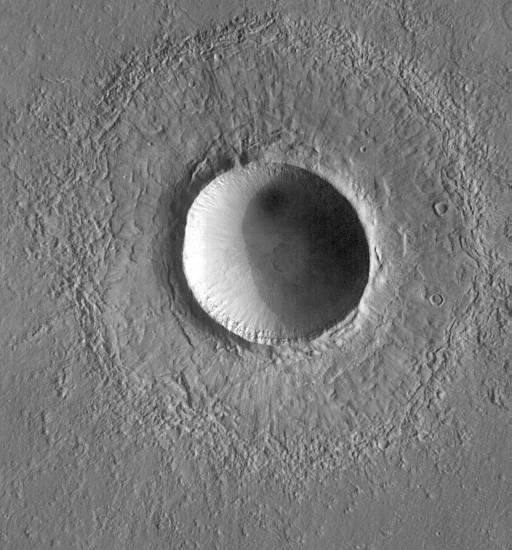
\includegraphics[width=.9\linewidth]{images/Gre13/Gre13_01.jpg} &
		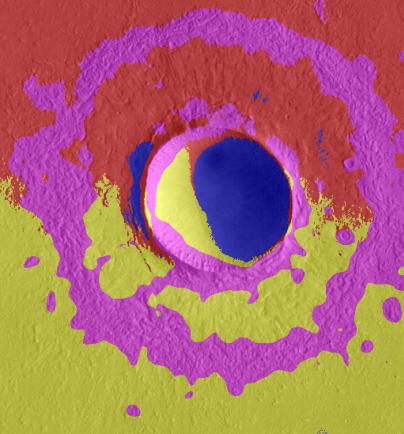
\includegraphics[width=.9\linewidth]{images/gen/filterbanks/Gre13_01.jpg_TSUGF.png} &
		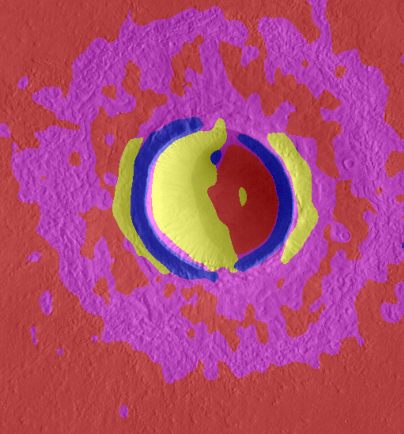
\includegraphics[width=.9\linewidth]{images/gen/filterbanks/Gre13_01.jpg_LM.png} &
		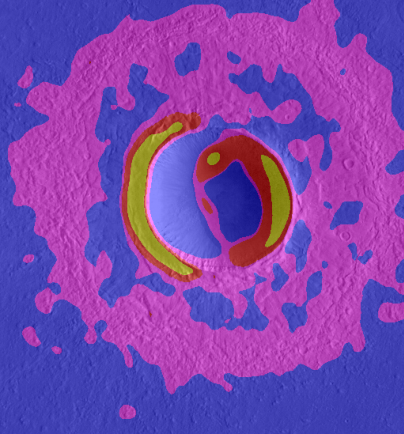
\includegraphics[width=.9\linewidth]{images/gen/filterbanks/Gre13_01.jpg_S.png} &
		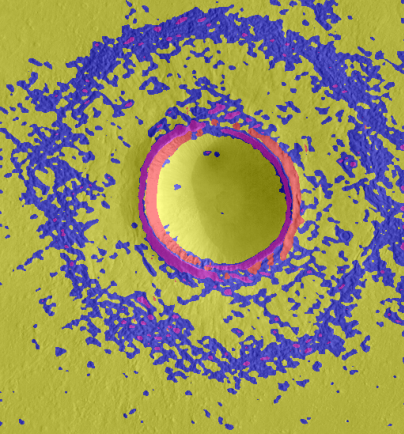
\includegraphics[width=.9\linewidth]{images/gen/filterbanks/Gre13_01.jpg_MR.png} \\
		
		Vulkan &
		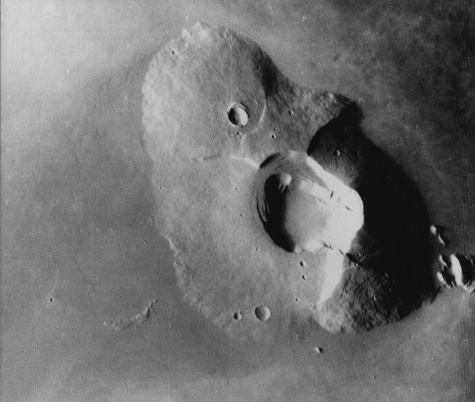
\includegraphics[width=.9\linewidth]{images/Gre13/Gre13_02.jpg} &
		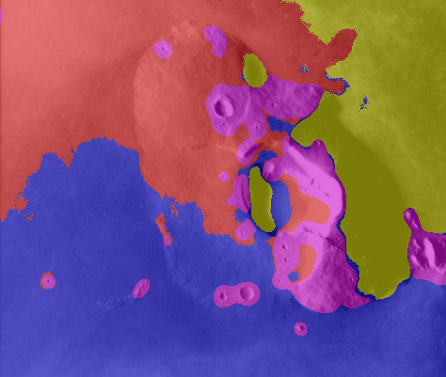
\includegraphics[width=.9\linewidth]{images/gen/filterbanks/Gre13_02.jpg_TSUGF.png} &
		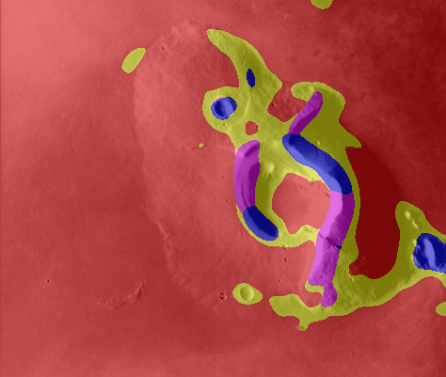
\includegraphics[width=.9\linewidth]{images/gen/filterbanks/Gre13_02.jpg_LM.png} &
		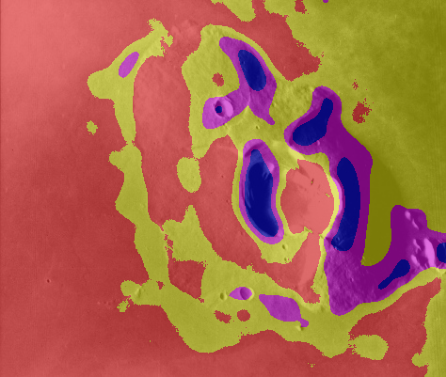
\includegraphics[width=.9\linewidth]{images/gen/filterbanks/Gre13_02.jpg_S.png} &
		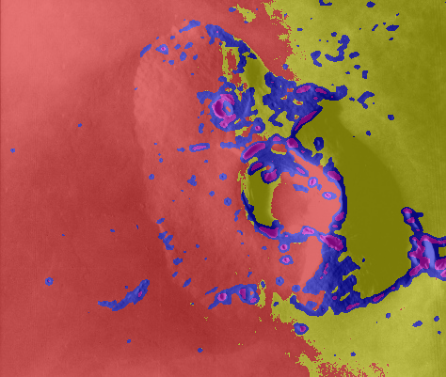
\includegraphics[width=.9\linewidth]{images/gen/filterbanks/Gre13_02.jpg_MR.png} \\
		
		Vulkan mit\newline strahlen-\newline förmigen Merkmalen &
		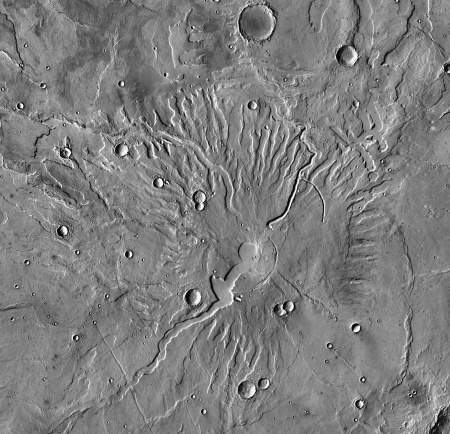
\includegraphics[width=.9\linewidth]{images/Gre13/Gre13_03.jpg} &
		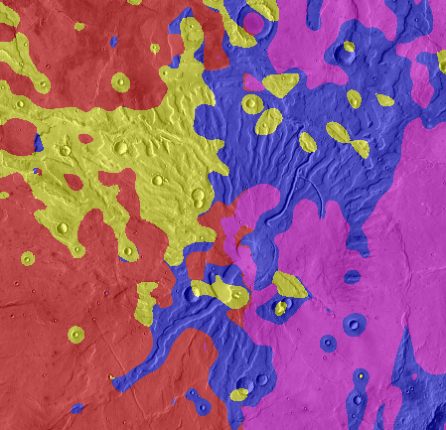
\includegraphics[width=.9\linewidth]{images/gen/filterbanks/Gre13_03.jpg_TSUGF.png} &
		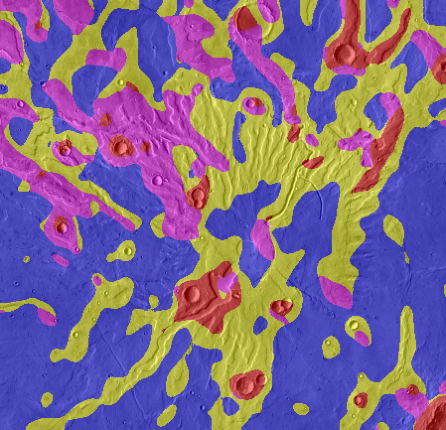
\includegraphics[width=.9\linewidth]{images/gen/filterbanks/Gre13_03.jpg_LM.png} &
		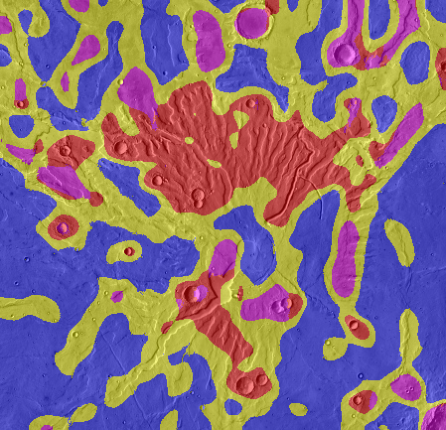
\includegraphics[width=.9\linewidth]{images/gen/filterbanks/Gre13_03.jpg_S.png} &
		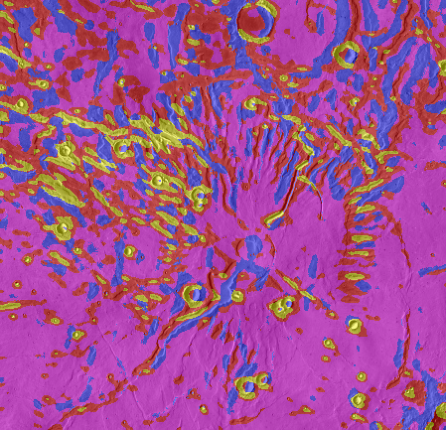
\includegraphics[width=.9\linewidth]{images/gen/filterbanks/Gre13_03.jpg_MR.png} \\
		
		Gletscher &
		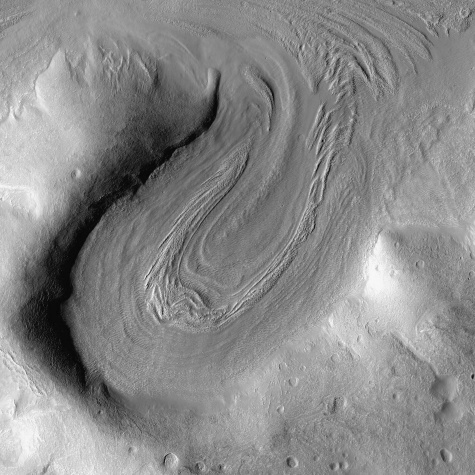
\includegraphics[width=.9\linewidth]{images/Gre13/Gre13_05.jpg} &
		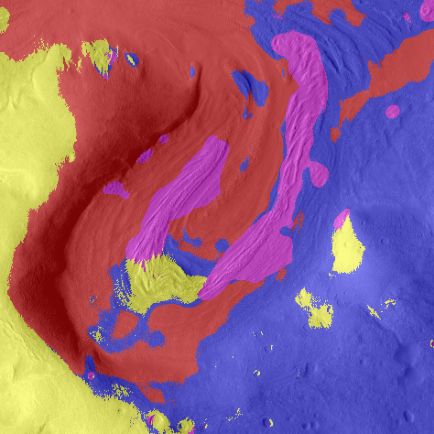
\includegraphics[width=.9\linewidth]{images/gen/filterbanks/Gre13_05.jpg_TSUGF.png} &
		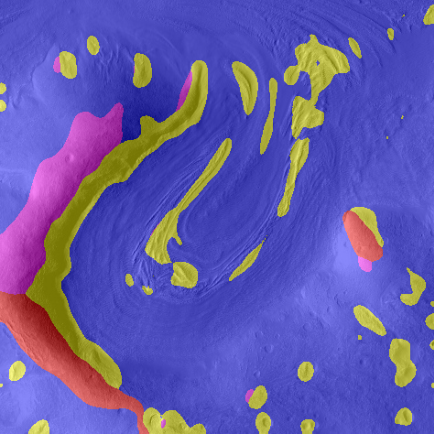
\includegraphics[width=.9\linewidth]{images/gen/filterbanks/Gre13_05.jpg_LM.png} &
		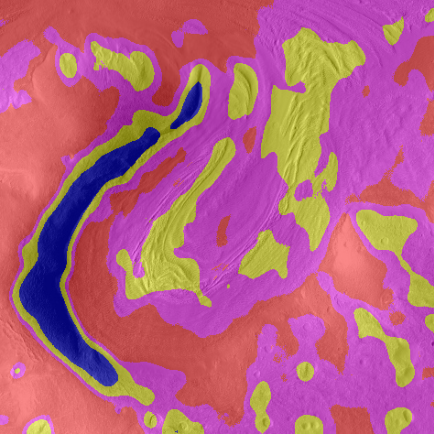
\includegraphics[width=.9\linewidth]{images/gen/filterbanks/Gre13_05.jpg_S.png} &
		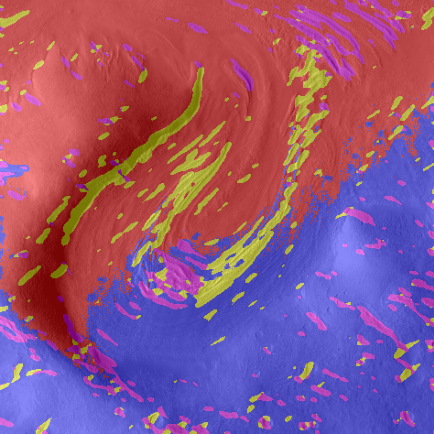
\includegraphics[width=.9\linewidth]{images/gen/filterbanks/Gre13_05.jpg_MR.png} \\
		\bottomrule
	\end{tabularx}
	\caption{Vergleich verschiedener Filterbänke auf Bildern der Marsoberfläche. Die Farben der jeweiligen Cluster wurden zufällig gewählt und sagen nichts über deren Inhalt aus. Alle Bilder wurden in vier Cluster eingeteilt.}
	\label{tab:filterbank_comparision}
\end{table}

\paragraph{Krater}
Neben dem eigentlichen Krater ist auf dieser Aufnahme der Ring aus gröberem Gestein ein wichtiges Merkmal. Dieser wird von allen Filterbänken zuverlässig erkannt, wenn auch mit einer unterschiedlichen Dicke: Die LM- und S-Filterbank selektieren dieses Gestein eher großzügig, die MR-Filterbank hingegen zeigt sehr enge Markierungen dieser Region.

Alle Filterbänke formen einen Ring (oder dessen Ansatz) auf dem Kraterrand, die Maximum Response-Filterbank erzeugt zwei konzentrische Ringe

Der Krater selbst wird von den Filterkombinationen nach \cite{jain_91} und der LM-Filterbank leider nur in Hell- und Dunkel-Regionen aufgeteilt, die S-Filterbank zeigt innerhalb des Kraters kein brauchbares Ergebnis. Eine Ausnahme stellt die Maximum-Response-Filterbank dar, welche neben den zwei erwähnten konzentrischen Clustern den Bereich innerhalb des Kraters als ein einziges Cluster erkennt. Dies zeugt von einer Invarianz gegenüber den Helligkeitswerten, da alle weiteren Filterbänke in diesem Bereich zwischen Licht- und Schattenregionen unterschieden haben. Die Maximum Response-Bank erzeugt in diesem Bereich das Resultat, welches sich wohl als bestes zur Weiterverarbeitung eignet, da sie unanfälliger für Helligkeitsveränderungen innerhalb eines Clusters ist und die Kraterränder am genauesten erfasst.

\paragraph{Vulkan}
Der Vulkanberg wird leider von keiner Filterbank optimal erkannt. Der äußere Rand wird nur von der S-Filterbank als ein Cluster erkannt, dies allerdings nicht sehr genau. Der rauere Bereich der Oberfläche, was kleinere Krater miteinbeschließt, wird vom MR-Filter am ehesten und genausten erkannt, auf dem zweiten Platz folgt die Filterbank nach \cite{jain_91}, welche zwar alle Krater in ein Cluster fügt (violett), allerdings eher gröber.

Die Vulkanmitte wird von keiner Filterbank erkannt, nur bei der MR-Bank lässt sich eine ringförmige, rauere Stelle um den Krater herum erahnen. Die anderen Filterbänke selektieren an dieser Stelle hauptsächlich nach den Helligkeitswerten. Außerdem ist interessant, dass der LM-Filter die Bergspitzen in vom Umfeld getrennte Cluster einteilt (blau und violett). Somit scheint es, als ließe sich diese Aufnahme über keine Filterbank gut clustern. Am ehesten eignet sich allerdings erneut die MR-Bank.

\paragraph{Vulkan mit strahlenförmigen Merkmalen}

Das Ziel bei der Nutzung dieser Marsaufnahme zur Analyse besteht daraus zu analysieren, mit welcher Filterbank die konzentrischen Strahlen am genauesten erkannt werden. Des Weiteren existieren auf der Aufnahme noch Krater, welche es separat einzuordnen gilt.

Die Filterbank nach \cite{jain_91} erkennt die gröberen Strukturen (Strahlen und Krater), fügt diese allerdings in dasselbe Cluster ein (gelb und blau).

Die LM-Filterbank scheint kein brauchbares Ergebnis zu produzieren, sie erkennt im Allgemeinen nur einige der Krater (rot) separat von deren Umfeld, die Strahlen sind nicht geeignet geclustert worden.

Die Schmid-Filterbank clustert einen Großteil der Strahlen gemeinsam in ein Cluster (rot). Die Krater hingegen sind nicht fest einer Clusterart zugewiesen, ein Großteil von ihnen befindet sich jedoch auch im roten Cluster.

Wie in den vorherigen Tests ist das Resultat der MR-Filterbank schon fast zu genau, die Cluster sind sehr fein gehalten. Im Gegensatz zu den Alternativen, werden hier die Krater relativ zuverlässig in gelbe Cluster eingeordnet, die Strahlen sind leider zu fein markiert, als dass man sie getrennt erkennen könnte. Dieses Phänomen könnte sich allerdings in der praktischen Anwendung zunutze gemacht werden, da dafür eine zu feine Initialisierung notwendig ist.

\paragraph{Gletscher}

Der Gletscher stellt im Bereich der Bildsegmentierung ein vergleichsweise schwieriges Problem dar, da er an vielen seiner Ränder keine feste Grenze zu benachbarten Regionen zeigt, nur links auf der Aufnahme ist er durch eine Hügelreihe strikt begrenzt. Diese Grenze wird von allen Filterbänken separat in ein oder mehrere getrennte Cluster unterteilt, mit Ausnahme der Filterbank nach \cite{jain_91}: Diese produziert kein geeignetes Ergebnis, nur die stärker erkennbaren \enquote{Streifen} werden gut erkannt (violett). Die LM-Filterbank erkennt zwar die Abgrenzung auf der linken Seite, allerdings keine anderen Regionen korrekt. Sie liefert bei diesem Bild das wohl schlechteste Resultat. Die Maximum-Response Methode und die Filterbank nach \cite{schmid_01} liefern zwar etwas bessere Ergebnisse, diese sind allerdings nicht ausreichend. Die MR-Bank erzeugt erneut sehr feine Cluster.

\paragraph{}
Zusammengefasst erzeugt aus dieser Auswahl an Filterbänden die Maximum Response-Methode von \cite{visgeo} das wohl am ehesten geeignete Resultat zur Weiterverarbeitung, da sie bei einem Großteil der Beispielbilder das beste Ergebnis produziert hat. Auf dem zweitem Platz folgt die Schmid-Filterbank.

\subsection{Größe der Filter}
\label{ssec:exp_filtersize}

% TODO WTF annotation

Es wird nun versucht, die Ergebnisse der Maximum Response-Filterbank zu verbessern, da diese in vorherigen Versuchen die besten Ergebnisse erzielt hat.

Bis jetzt wurden die Marsaufnahmen aus \cite[Kap.~7]{greeley_13} genutzt, da diese möglichst diverse Oberflächenstrukturen- und Merkmale abdecken. Von dieser Stelle an müssen allerdings Marsaufnahmen genutzt werden, bei denen die Auflösung bekannt ist, somit scheiden die genutzten leider aus. Stattdessen werden Ausschnitte aus der Aufnahme \texttt{P03\_002147\_1865\_XI\_06N208W} der Context Camera des Mars Reconnaissance Orbiters genutzt. Auch diese wurden so ausgewählt, dass sie möglichst diverse Strukturen und Texturen aufweisen. Ein weiterer Vorteil der Nutzung dieser Bilder besteht daraus, dass die Clusteringalgorithmen nun an realitätsnähreren Daten getestet werden können, statt an isolierten Aufnahmen einzelner Besonderheiten der Oberfläche. Die Ergebnisse sind in \tablename~\ref{tab:filterbank_sizes} zu sehen. Als Startwert wurde ein Skalierungsfaktor $s=1$ betrachtet, angewandt auf die vorgestellten, quadratischen Filter mit einer originalen Kantenlänge von \SI{49}{\pixel}.  Dieser wurde nach oben und unten hin in Schritten von $\Delta s=0.25$ verändert, und mit der skalierten MR-Filterbank ein neues Clustering der vier Ausschnitte erstellt. Die Eingabebilder sind quadratisch und besitzen eine Seitenlänge von \SI{650}{\pixel} bei einer Auflösung von \SI{6,17}{\meter\per\pixel}. Jedes der Eingabebilder wurde erneut in vier Bereiche eingeteilt, die Farben sind zur Veranschaulichung zufällig gewählt, da der Algorithmus zwar in Segmente unterteilen kann, allerdings nicht bestimmen kann, was diese Segmente enthalten.

\begin{table}[h!]
	\setlength\tabcolsep{0pt}
	\begin{tabularx}{\textwidth}{>{\centering}m{0.05\textwidth}
			>{\centering}m{0.136\textwidth}
			>{\centering}m{0.136\textwidth}
			>{\centering}m{0.136\textwidth}
			>{\centering}m{0.136\textwidth}
			>{\centering}m{0.136\textwidth}
			>{\centering}m{0.136\textwidth}
			>{\centering\arraybackslash}m{0.136\textwidth}}
		\toprule
		Bez. &
		Eingabe & 
		$s=0,25$ &
		$s=0,50$ &
		$s=0,75$ &
		$s=1,00$ &
		$s=1,25$ &
		$s=1,50$ \\
		\midrule
		
		\texttt{a)} &
		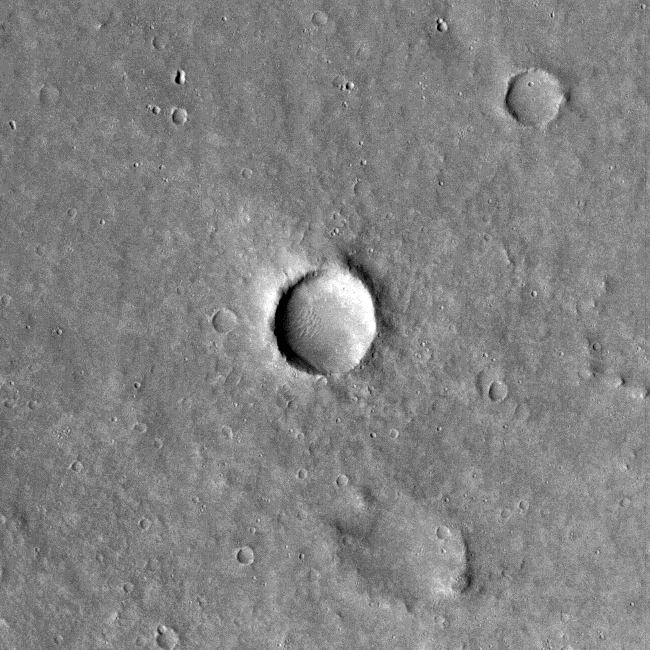
\includegraphics[width=0.9\linewidth]{images/p03/p03_01.png} &
		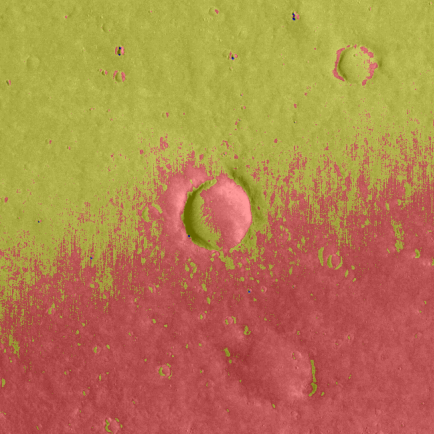
\includegraphics[width=0.9\linewidth]{images/gen/filter_size/p03_01.png_0.25.png} &
		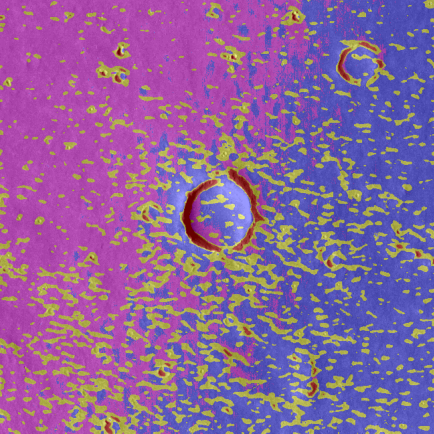
\includegraphics[width=0.9\linewidth]{images/gen/filter_size/p03_01.png_0.50.png} &
		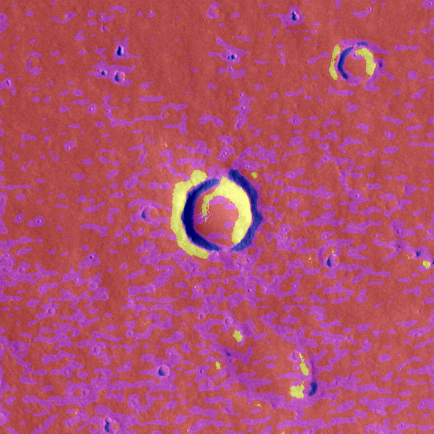
\includegraphics[width=0.9\linewidth]{images/gen/filter_size/p03_01.png_0.75.png} &
		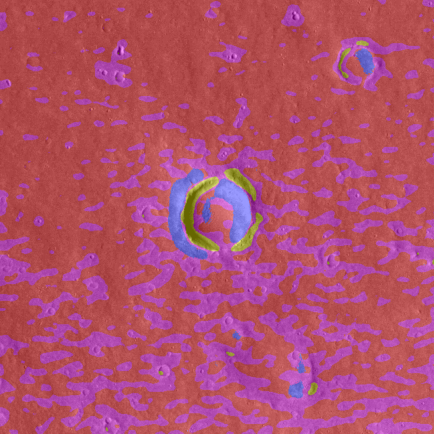
\includegraphics[width=0.9\linewidth]{images/gen/filter_size/p03_01.png_1.00.png} &
		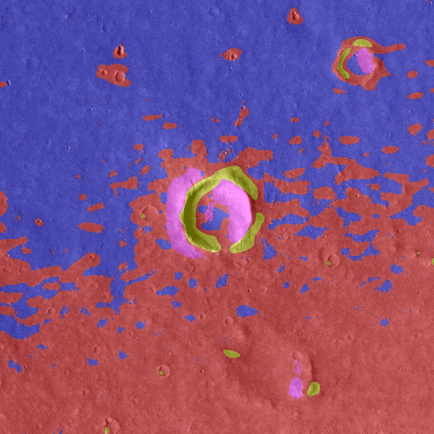
\includegraphics[width=0.9\linewidth]{images/gen/filter_size/p03_01.png_1.25.png} &
		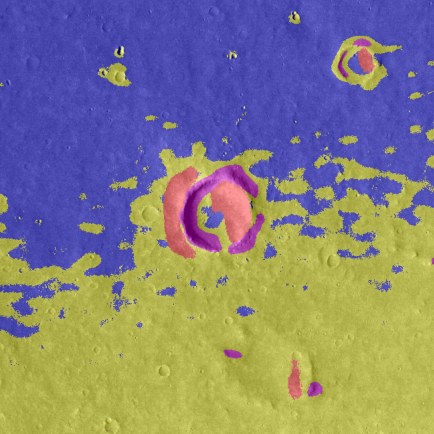
\includegraphics[width=0.9\linewidth]{images/gen/filter_size/p03_01.png_1.50.png} \\
		\texttt{b)} &
		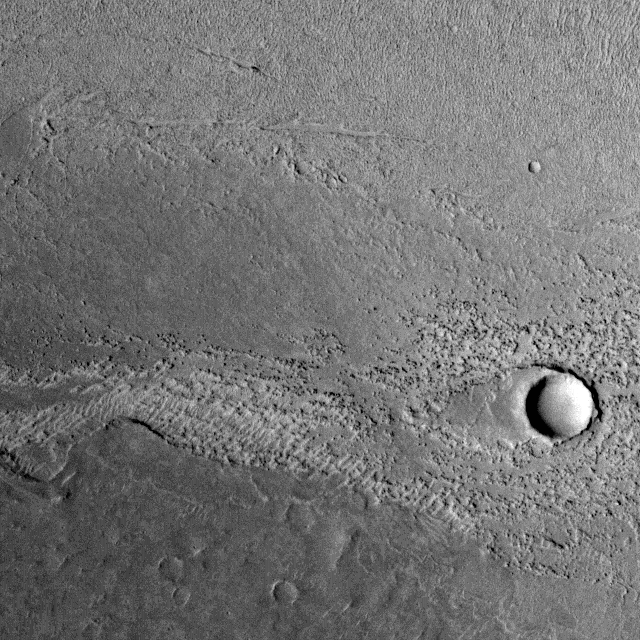
\includegraphics[width=0.9\linewidth]{images/p03/p03_02.png} &
		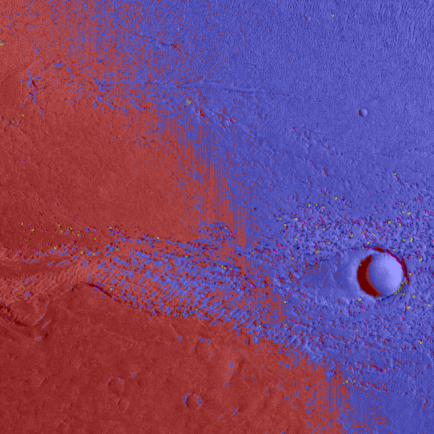
\includegraphics[width=0.9\linewidth]{images/gen/filter_size/p03_02.png_0.25.png} &
		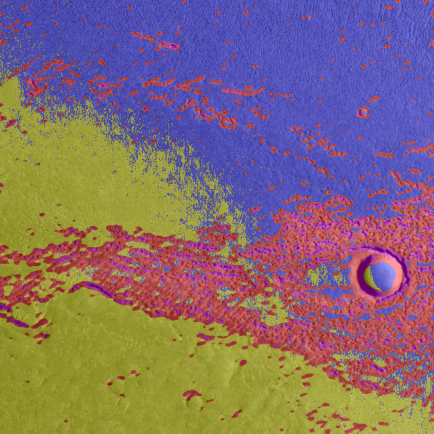
\includegraphics[width=0.9\linewidth]{images/gen/filter_size/p03_02.png_0.50.png} &
		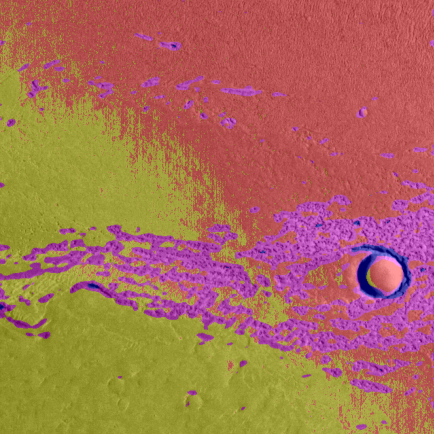
\includegraphics[width=0.9\linewidth]{images/gen/filter_size/p03_02.png_0.75.png} &
		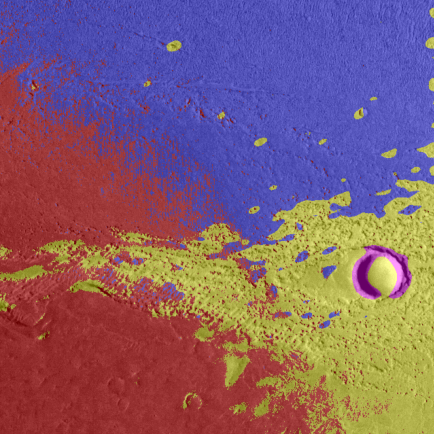
\includegraphics[width=0.9\linewidth]{images/gen/filter_size/p03_02.png_1.00.png} &
		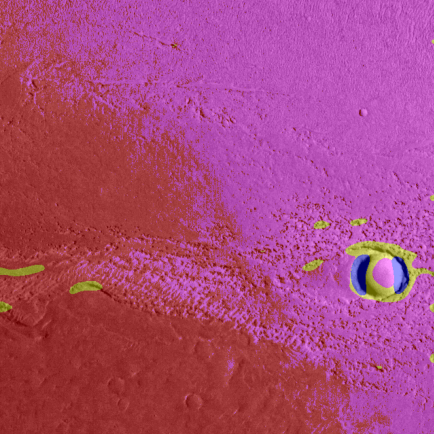
\includegraphics[width=0.9\linewidth]{images/gen/filter_size/p03_02.png_1.25.png} &
		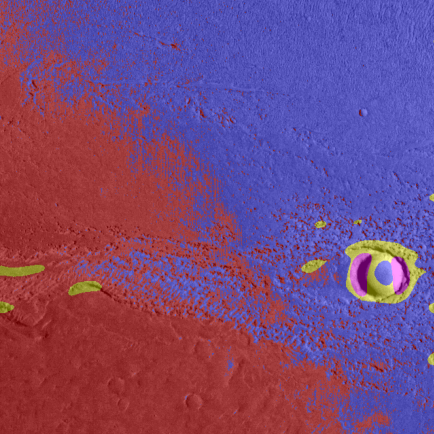
\includegraphics[width=0.9\linewidth]{images/gen/filter_size/p03_02.png_1.50.png} \\
		\texttt{c)} &
		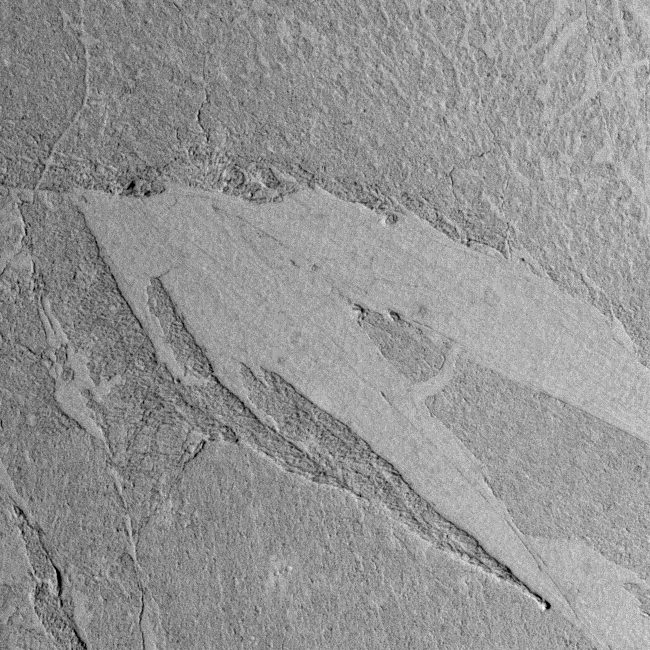
\includegraphics[width=0.9\linewidth]{images/p03/p03_03.png} &
		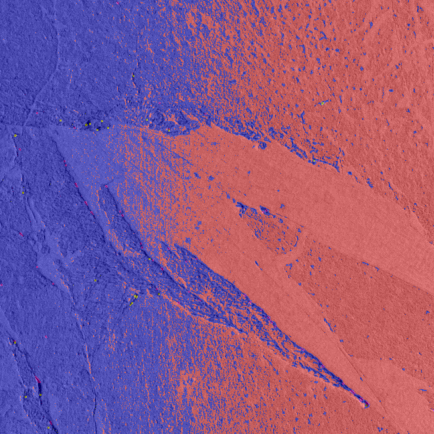
\includegraphics[width=0.9\linewidth]{images/gen/filter_size/p03_03.png_0.25.png} &
		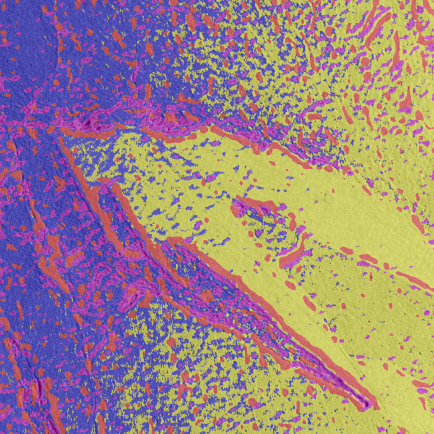
\includegraphics[width=0.9\linewidth]{images/gen/filter_size/p03_03.png_0.50.png} &
		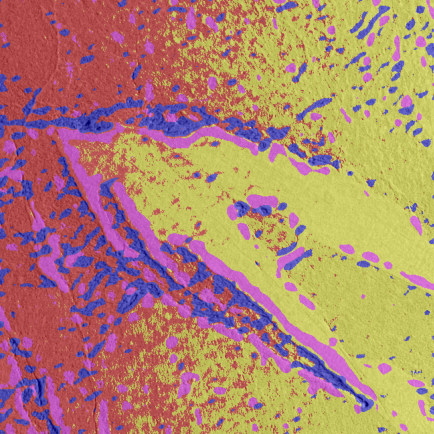
\includegraphics[width=0.9\linewidth]{images/gen/filter_size/p03_03.png_0.75.png} &
		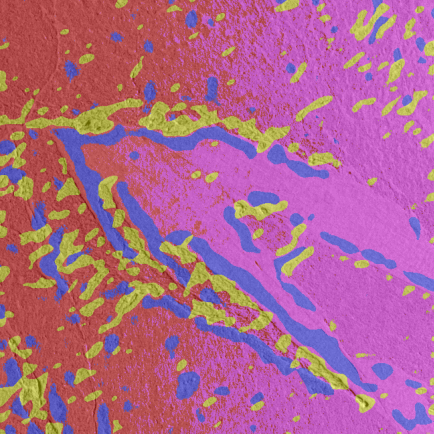
\includegraphics[width=0.9\linewidth]{images/gen/filter_size/p03_03.png_1.00.png} &
		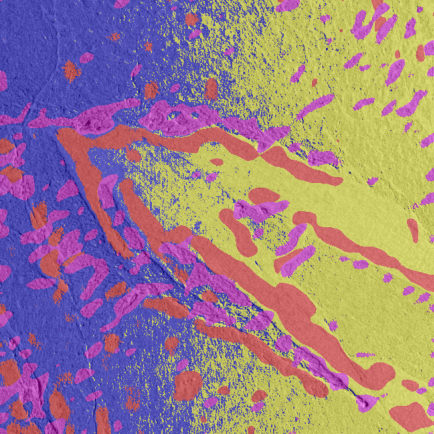
\includegraphics[width=0.9\linewidth]{images/gen/filter_size/p03_03.png_1.25.png} &
		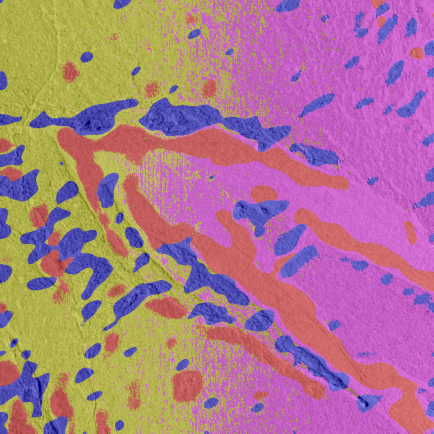
\includegraphics[width=0.9\linewidth]{images/gen/filter_size/p03_03.png_1.50.png} \\
		\texttt{d)} &
		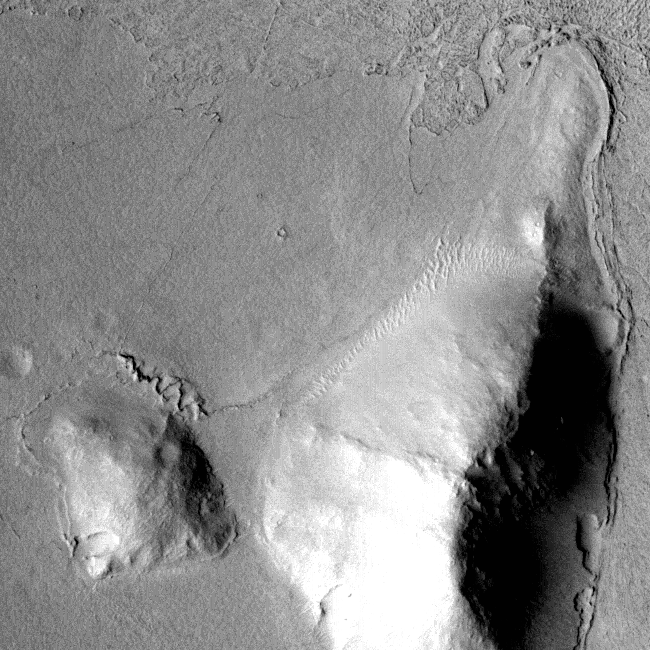
\includegraphics[width=0.9\linewidth]{images/p03/p03_04.png} &
		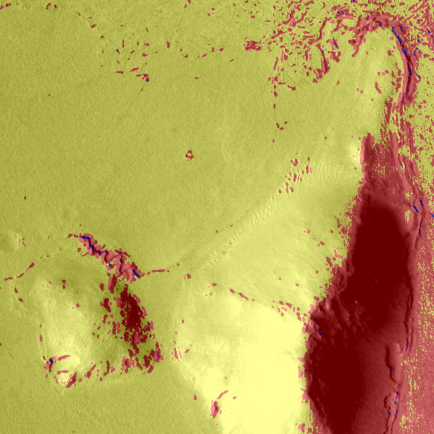
\includegraphics[width=0.9\linewidth]{images/gen/filter_size/p03_04.png_0.25.png} &
		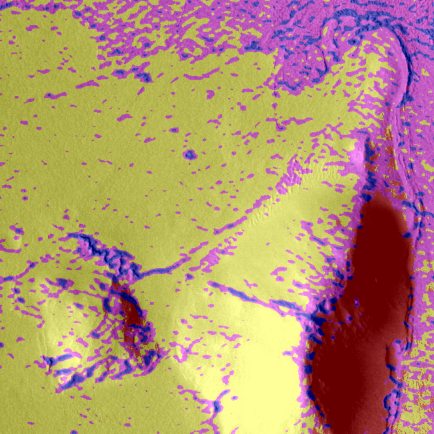
\includegraphics[width=0.9\linewidth]{images/gen/filter_size/p03_04.png_0.50.png} &
		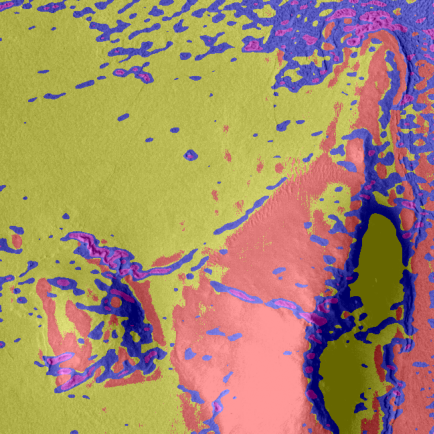
\includegraphics[width=0.9\linewidth]{images/gen/filter_size/p03_04.png_0.75.png} &
		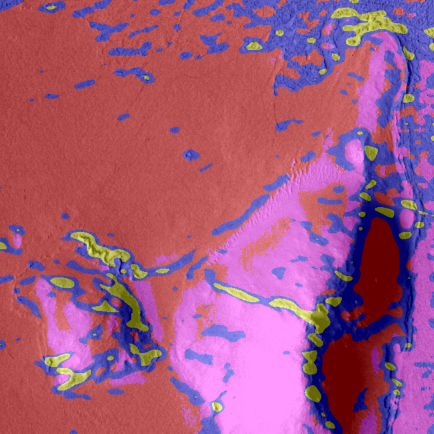
\includegraphics[width=0.9\linewidth]{images/gen/filter_size/p03_04.png_1.00.png} &
		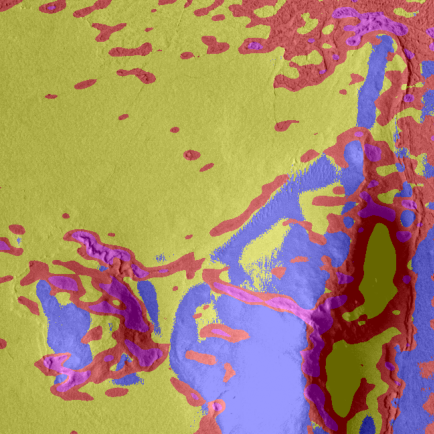
\includegraphics[width=0.9\linewidth]{images/gen/filter_size/p03_04.png_1.25.png} &
		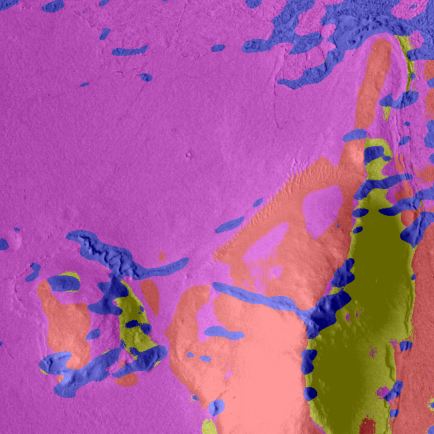
\includegraphics[width=0.9\linewidth]{images/gen/filter_size/p03_04.png_1.50.png} \\
		\bottomrule
	\end{tabularx}
	\caption{Vergleich verschiedener Skalierungen der MR-Filterbank auf Bildern der Marsoberfläche. Die Farben der jeweiligen Cluster wurden zufällig gewählt und sagen nichts über deren Inhalt aus. Alle Bilder wurden in vier Cluster eingeteilt.}
	\label{tab:filterbank_sizes}
\end{table}


Von hier an gilt in allen Vergleichen von Segmentierungen: Die erste Zeile der Tabelle entspricht der ersten Aufnahme, die zweile Zeile entspricht der zweiten Aufnahme, \etc.

\paragraph{Skalierungsfaktor $s=0,25$}

Auf Aufnahme \texttt{a)} ist, vergleichbar mit den Beispielaufnahmen aus dem letzten Abschnitt, ein runder Krater zentriert zu sehen. Die geringe Skalierung mit dem Faktor $s=0.25$ führt dazu, dass die jeweiligen Filter zu klein sind, um die Strukturen der Oberfläche zu erkennen, somit sieht diese Aufnahme aus, als wäre nur anhand ihrer Helligkeitswerten geclustert worden. Das gleiche gilt auch für die Aufnahmen \texttt{b)} und \texttt{d)}.

Aufnahme \texttt{c)} stellt eine relativ ebenmäßige Fläche in einem Umfeld von gröberer Oberfläche dar. Dort scheint es, als gäbe es nicht genug Kontrast um nach den Helligkeitswerten zu clustern, der Algorithmus erstellt eine Filterung anhand der X- und Y-Koordinaten. Bei allen Aufnahmen werden nur zwei wirkliche Cluster erstellt, die letzten zwei Cluster die erstellt werden sollten bestehen nur aus jeweils wenigen Pixeln.

Dieser Skalierungsfaktor produziert keine brauchbaren Ergebnisse.

\paragraph{Skalierungsfaktor $s=0,50$}

Wie zu Erwarten führt die genutzte, noch relativ geringe Skalierung der Filterbank mit $s=0,50$ zu vielen kleineren Clustern, in diesem Fall auf Aufnahme \texttt{a)} deutlich erkennbar anhand der gelb markierten Flächen. Obwohl es auf den ersten Blick scheint, als würden die Kraterränder erkannt werden, werden durch die Filterbank bei dieser Skalierung nur die dunkleren Bereiche, in diesem Fall die Schatten, welche die erhöhten Kraterränder werfen, erkannt. Auf dieser Aufnahme führt dies zwar zu einer vergleichsweise guten Approxmimation der Krater, sobald anderweitige Schatten hinzukommen, produziert diese Skalierung allerdings keine geeigneten Resultate.

Das selbe Phänomen tritt bei der Aufnahme in der zweiten Zeile von oben auf, auch dort wird stark anhand der Helligkeitswerte geclustert, erkennbar insbesondere an den violetten Bereichen an den Kraterrändern. Bei diesem Bild wird allerdings auch trotz der kleineren Skalierung das raue Gebiet, welches sich horizontal durch das Bild erstreckt, in ein (rot gefärbtes) Cluster eingeteilt. Auch hier werden allerdings dunklerere Bereiche (wie die Kraterränder) in separate (violett gefärbte) Cluster eingeteilt.

Auf Aufnahme \texttt{c)} wird bei der genutzten Skalierung die feinere Fläche größtenteils als ein (gelb gefärbtes) Cluster dargestellt, separat dazu sind in rot die Übergänge zwischen den Regionen gekennzeichnet. Die gröberen Flächen in den äußeren Bereichen werden nicht zuverlässig in das selbe Cluster eingeordnet.

Die letzte Testaufnahme, bestehend aus zwei Hügeln \bzw Bergen, stellt durch die stark und wenig belichteten Flächen an den Hängen eine der größten Herausforderungen für den Clusteringalgorithmus dar. An diesen Stellen ist der Kontrast des Bildes sehr gering, sodass kaum noch Texturen erkannt werden, anhand derer geclustert werden könnte. Wie zu erwarten werden die dunklen Flächen in ein einzelnes (rotes) Cluster kombiniert. Kleine Hügelketten hingegen werden zuverlässig in zusammengehörige Cluster eingeteilt, welches auf diesen Aufnahmen blau markiert ist. Die beleuchteten Seiten der Hügel werden bei dieser Skalierung leider nicht von der allgemeinen Marsoberfläche unterschieden, höchstens der Fuß des Berges kann durch die violette Färbung erahnt werden.

Dieser Skalierungsfaktor führt zu vergleichsweise guten Clusteringergebnissen.

\paragraph{Skalierungsfaktor $s=0,75$}

Dieser Skalierungsfaktor führt beim Clustering des obersten Bildes, Aufnahme \texttt{a)}, zu Resultaten, welche vergleichbar mit denen des Faktors $s=0,5$ sind. Die Ränder der Krater werden allerdings getrennt in helle und dunkle Regionen eingeteilt, die Cluster im äußeren Bereich sind größer und gröber.

Auf Aufnahme \texttt{b)} wird die horizontale rauere Region sehr gut in ein eigenes Cluster eingeteilt, selbiges gilt für die Kraterränder. Auf dieser Aufnahme erscheint der Skalierungsfaktor $s=0,75$ für diese Filterbank optimal.

Die vorletzte Aufnahme, Aufnahme \texttt{c)}, unterscheidet sich bis auf die gröberen, größeren Cluster in den äußeren Bereichen nicht wesentlich von der vorherigen Skalierung.

Bei der untersten Aufnahme führt die größere Skalierung zu einem uniformen Clusterings des beleuchteten Berghangs, er wird als eine große Fläche erkannt. Die dunkle Seite hingegen wird in zwei Cluster unterteilt: Die eigentliche dunkle Seite des Berges, und die Stellen, welche zu unterbelichtet sind, um aus ihnen eine Textur zu erkennen.

Insgesamt scheint sich dieser Skalierungsfaktor auch zum texturbasierten Clustering zu eignen.

\paragraph{Skalierungsfaktor $s=1,00$}

Während bei diesem Skalierungsfaktor auf Aufnahme \texttt{a)} der größere, mittige Krater relativ gut durch ein gelbes kreisförmiges Cluster gekennzeichnet wird, wird der kleinere Krater nicht zuverlässig erkannt. Bei diesem gehen die Cluster in umlegende Gebiete über, als wäre dieser Krater nur eine etwas rauere Oberflächenstruktur.

Bei Aufnahme \texttt{b)} wird wie zuvor der Krater erfolgreich separat in ein Cluster eingeteilt, die Begrenzungen der gröberen Struktur, welche sich durch das Bild zieht, geht allerdings verloren. Diese Region wird leider im rechten Teil des Bildes sehr weitläufig erkannt.

In Testbild \texttt{c)} werden die gröberen Hügelketten am Rand des helleren Bereiches zwar erkannt (gelb markiert), und die Übergangsstellen zwischen zwei Regionen werden in ein blaues Cluster zusammengefügt, alle anderen Regionen sind allerdings nicht voneinander getrennt worden.

Bild \texttt{d)} wird bei dieser Skalierung fast identisch zu der Skalierung mit $s=0,75$ geclustert.

Zusammengefasst ist diese Skalierung schon zu grob um so gute Ergebnisse wie die vorherigen zu erreichen.

\paragraph{Skalierungsfaktor $s=1,25$ und $s=1,50$}

Da diese beiden Skalierungsfaktoren zu fast identischen Clusterverteilungen führen, werden sie in einen Abschnitt zusammengefasst.

Bei diesen Skalierungen werden im oberen, weniger rauen Bereich der Aufnahme \texttt{a)} die vereinzelten Krater wie gewollt erkannt, sie versagen allerdings im unteren, gröberen Bereich, wo sie nur ein großes Cluster erstellen. Der Krater wird nur anhand von starken Helligkeitsdifferenzen erkannt, welche in der gesamten Ausgabe gelb bei $s=1,25$, \bzw violett bei $s=1,5$ markiert wurden. 

Selbiges gilt im Bezug auf die starken Helligkeitsdifferenzen in Aufnahme \texttt{b)}.

Bei Aufnahme \texttt{c)} wird von beiden Skalierungsfaktoren kein brauchbares Resultat produziert, man kann höchstens erahnen, dass die gelb \bzw violett gefärbten Regionen besonders kontrastarme, also glatte Flächen darstellen sollen.

Beim Clusteringergebnis der letzten Aufnahme unterschieden sich die beiden Skalierungsfaktoren erstmals stärker: Bei $s=1,25$ gleicht das Ergebnis dem des vorherigen Clusterings: Kleinere Bergregionen und rauere Oberflächenstrukturen werden getrennt voneinander erkannt, Flächen mit weniger oder (aufgrund von Unterbelichtung) keiner werden auch in ein großes Cluster hinzugefügt. Der Faktor $s=1,5$ scheint selbst bei diesem Bild zu groß zu sein, bis auf die Hügelketten mit starker Helligkeitsdifferenz wird die Aufnahme nur anhand ihrer Helligkeitswerte geclustert.

Diese Skalierungsfaktoren führen also zu Filtern, welche eine zu große Kantenlänge besitzen um brauchbare Resultate zu produzieren, da die Muster innerhalb einer Oberflächentextur eine wesentlich geringere Entfernung besitzen, nach welcher sie sich wiederholen.

\paragraph{}
Aus diesen Ergebnissen lässt sich schlussfolgern, dass sich die Skalierungsfaktoren $s=0,5$ und $s=0,75$ bei diesen Eingabedaten die besten Resultate liefert. Da durch die nachfolgende Weiterverarbeitung durch den Algorithmus nach Kanezaki eine hohe Anzahl an Clustern benötigt wird, diese aber nicht zu klein und verstreut ausfallen sollten, wird von nun an ein Skalierungsfaktor von $s=0,75$ genutzt.

\subsection{Gewichtung der Parameter}
\label{ssec:exp_filterweight}

Wie in Unterabschnitt~\ref{ssec:initialization_filterweight} erläutert, spielt die Gewichtung der Komponenten des Datenwürfels, welcher zum Clustering durch k-Means genutzt wird eine wichtige Rolle. In den Abbildungen~\ref{tab:filterbank_weights_pos} und \ref{tab:filterbank_weights_col} die Resultate des Clusterings mit unterschiedlichen Werten für diese jeweiligen Gewichtungen zu sehen. Die Skalierung der Filter beträgt $s=0,5$, da im vorherigen Unterabschnitt festgestellt wurde, dass dieser Wert relativ gute Ergebnisse liefert.

\begin{table}[h!]
	\setlength\tabcolsep{0pt}
	\begin{tabularx}{\textwidth}{>{\centering}m{0.05\textwidth}
		>{\centering}m{0.136\textwidth}
		>{\centering}m{0.136\textwidth}
		>{\centering}m{0.136\textwidth}
		>{\centering}m{0.136\textwidth}
		>{\centering}m{0.136\textwidth}
		>{\centering}m{0.136\textwidth}
		>{\centering\arraybackslash}m{0.136\textwidth}}
	
		\toprule
		Bez. &
		Eingabe & 
		$w_p=0,00$ &
		$w_p=0,33$ &
		$w_p=0,66$ &
		$w_p=1,00$ &
		$w_p=1,33$ &
		$w_p=1,66$ \\
		\midrule
		\texttt{a)} &
		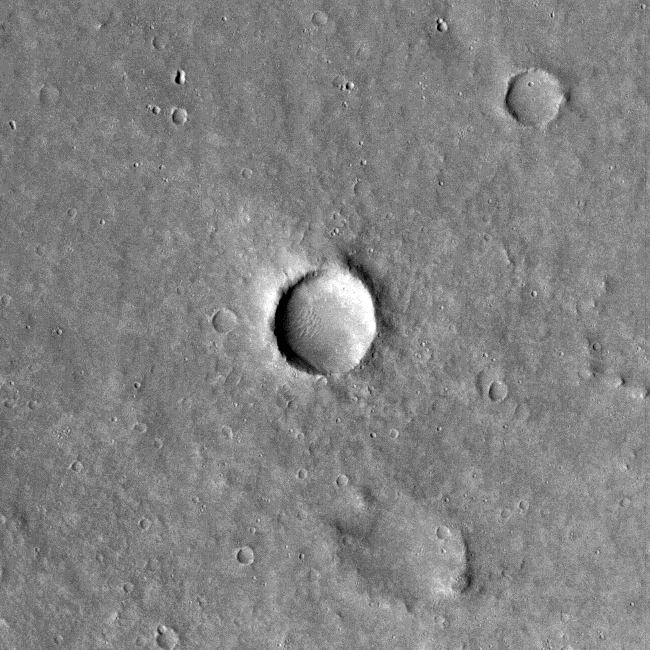
\includegraphics[width=0.9\linewidth]{images/p03/p03_01.png} &
		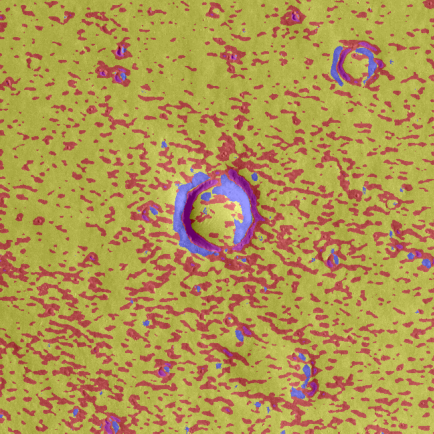
\includegraphics[width=0.9\linewidth]{images/gen/spatial_weight/p03_01.png_0.00.png} &
		\includegraphics[width=0.9\linewidth]{images/gen/spatial_weight/p03_01.png_0.33.png} &
		\includegraphics[width=0.9\linewidth]{images/gen/spatial_weight/p03_01.png_0.66.png} &
		\includegraphics[width=0.9\linewidth]{images/gen/spatial_weight/p03_01.png_1.00.png} &
		\includegraphics[width=0.9\linewidth]{images/gen/spatial_weight/p03_01.png_1.33.png} &
		\includegraphics[width=0.9\linewidth]{images/gen/spatial_weight/p03_01.png_1.66.png} \\
		\texttt{b)} &
		\includegraphics[width=0.9\linewidth]{images/p03/p03_02.png} &
		\includegraphics[width=0.9\linewidth]{images/gen/spatial_weight/p03_02.png_0.00.png} &
		\includegraphics[width=0.9\linewidth]{images/gen/spatial_weight/p03_02.png_0.33.png} &
		\includegraphics[width=0.9\linewidth]{images/gen/spatial_weight/p03_02.png_0.66.png} &
		\includegraphics[width=0.9\linewidth]{images/gen/spatial_weight/p03_02.png_1.00.png} &
		\includegraphics[width=0.9\linewidth]{images/gen/spatial_weight/p03_02.png_1.33.png} &
		\includegraphics[width=0.9\linewidth]{images/gen/spatial_weight/p03_02.png_1.66.png} \\
		\texttt{c)} &
		\includegraphics[width=0.9\linewidth]{images/p03/p03_03.png} &
		\includegraphics[width=0.9\linewidth]{images/gen/spatial_weight/p03_03.png_0.00.png} &
		\includegraphics[width=0.9\linewidth]{images/gen/spatial_weight/p03_03.png_0.33.png} &
		\includegraphics[width=0.9\linewidth]{images/gen/spatial_weight/p03_03.png_0.66.png} &
		\includegraphics[width=0.9\linewidth]{images/gen/spatial_weight/p03_03.png_1.00.png} &
		\includegraphics[width=0.9\linewidth]{images/gen/spatial_weight/p03_03.png_1.33.png} &
		\includegraphics[width=0.9\linewidth]{images/gen/spatial_weight/p03_03.png_1.66.png} \\
		\texttt{d)} &
		\includegraphics[width=0.9\linewidth]{images/p03/p03_04.png} &
		\includegraphics[width=0.9\linewidth]{images/gen/spatial_weight/p03_04.png_0.00.png} &
		\includegraphics[width=0.9\linewidth]{images/gen/spatial_weight/p03_04.png_0.33.png} &
		\includegraphics[width=0.9\linewidth]{images/gen/spatial_weight/p03_04.png_0.66.png} &
		\includegraphics[width=0.9\linewidth]{images/gen/spatial_weight/p03_04.png_1.00.png} &
		\includegraphics[width=0.9\linewidth]{images/gen/spatial_weight/p03_04.png_1.33.png} &
		\includegraphics[width=0.9\linewidth]{images/gen/spatial_weight/p03_04.png_1.66.png} \\
		\bottomrule
	\end{tabularx}
	\caption{Vergleich verschiedener Gewichtungen der Koordinaten beim Clustering der jeweiligen Eingabedateien. Die Farben der jeweilgen Cluster wurden zufällig gewählt. Alle Bilder wurden in vier Cluster eingeteilt.}
	\label{tab:filterbank_weights_pos}
\end{table}

\paragraph{Gewichtung der Koordinaten}
Das Hinzufügen der X- und Y-Koordinaten zu dem Datenwürfel ist ursprünglich aus dem Grund geschehen, dass ein gegebener räumlicher Bezug zwischen unterschiedlichen Pixeln beim Clustering berücksichtigt werden kann (\vgl Unterabschnitt~\ref{ssec:tsugf}; \cite{jain_91}). Aus den Clusteringergebnissen in \tablename~\ref{tab:filterbank_weights_pos} allerdings lässt sich erkennen, dass dieser räumliche Bezug in diesem Anwendungsfall nicht außerordentlich hilfreich ist: Bei einer Gewichtung von $w_p\geq1,33$ lässt sich eindeutig erkennen, dass der allgemeine Bodenbereich auf allen Aufnahmen zu stark anhand seiner Positionen eingeteilt wird, es entstehen Cluster in den Ecken der Aufnahmen, welche sich ins Zentrum erstrecken. Unter diesem starken Einfluss nimmt zusätzlich die relative Wichtigkeit der ähnlichen Textur ab.

Wird nun ein geringerer Wert für $w_p$ betrachtet, so erkennt man für Werte mit $w_p\leq0,66$ keinen Starken Unterschied bei wechselnden Gewichtungen. Dies ist insbesondere bei $w_p=0$ signifikant, da dort der räumliche Bezug der einzelnen Pixel zueinander bei der Berechnung des Clusterings zwar komplett ignoriert wird, das eigentliche Ergebnis sich, bis auf etwas kleinere Cluster in den merkmalsarmen Bereichen, aber kaum verändert. Dies lässt sich darauf zurückführen, dass das Hinzufügen des räumlichen Bezuges ursprünglich den Grund hatte, dass auf \enquote{normalen} Fotografien die vorkommenden Cluster meistens nur ein einziges mal an einem räumlich begrenzten Ort vorhanden sind, so sind \zB bei der Aufnahme aus \figurename~\ref{fig:tsugf_optim} aus Unterabschnitt~\ref{ssec:tsugf} die kleineren Korallen im linken Hintergrund nur an dieser Stelle vorhanden und ließen sich durch ein weit ausgedehntes Cluster zusammenfassen. Bei den aktuell genutzten Aufnahmen hingegen ist dies nicht der Fall, eine auftretende Oberflächenstruktur, wie \zB ein Krater kann an verschieden Stellen ohne räumlichen Bezug zueinander auftreten.
Die Nutzung der Positionwerte hat allerdings einen Vorteil: Sie sorgt dafür die Clustergrößen nicht zu klein und fragmentiert werden zu lassen, indem sie eine Relation mit benachbarten Pixeln erzeugt, welche der k-Means Algorithmus berücksichtigt.

Aus diesem Grund macht es Sinn, die Koordinatenbeträge der Pixel relativ gering zu gewichten, um dafür zu sorgen, dass das texturbasierte Clustering möglicht positionsinvariant operiert, aber auch nicht so gering, dass viele fragmentierte Cluster entstehen. Anhand von \tablename~\ref{tab:filterbank_weights_pos} ist erkennbar, dass ein Wert von  $w_p=0,66$ sich in diesem Fall sehr gut eignet, ein brauchbares Clusterergebnis zu erstellen.

\paragraph{Gewichtungen der Farb-/Helligkeitswerte}
Die hier folgenden Clusteringergebnisse wurden mit den zuvor bestimmten optimalen Parametern erstellt.

In der originalen Ausarbeitung des texturbasierten Clusterings \cite{jain_91} werden nur zwei Ebenen für die jeweiligen X- und Y-Koordinaten hinzugefügt. Es steht also an dieser Stelle offen, ob das Hinzufügen der Farb- \bzw Helligkeitsdimension zum Datenwürfel zu besseren Ergebnissen führt. Dazu wurde der vorgestellte Algorithmus mit unterschiedlichen Werten für die Gewichtung der Helligkeitswerte $w_c$ auf den bekannten Beispielbildern ausgeführt. Die Resultate dieses Experimentes sind in \tablename~\ref{tab:filterbank_weights_col} dargestellt.

\begin{table}[h!]
	\setlength\tabcolsep{0pt}
	\begin{tabularx}{\textwidth}{>{\centering}m{0.05\textwidth}
			>{\centering}m{0.136\textwidth}
			>{\centering}m{0.136\textwidth}
			>{\centering}m{0.136\textwidth}
			>{\centering}m{0.136\textwidth}
			>{\centering}m{0.136\textwidth}
			>{\centering}m{0.136\textwidth}
			>{\centering\arraybackslash}m{0.136\textwidth}}
		\toprule
		Bez. &
		Eingabe & 
		$w_c=0,00$ &
		$w_c=0,33$ &
		$w_c=0,66$ &
		$w_c=1,00$ &
		$w_c=1,33$ &
		$w_c=1,66$ \\
		
		\midrule
		\texttt{a)} &
		\includegraphics[width=0.9\linewidth]{images/p03/p03_01.png} &
		\includegraphics[width=0.9\linewidth]{images/gen/color_weight/p03_01.png_0.00.png} &
		\includegraphics[width=0.9\linewidth]{images/gen/color_weight/p03_01.png_0.33.png} &
		\includegraphics[width=0.9\linewidth]{images/gen/color_weight/p03_01.png_0.66.png} &
		\includegraphics[width=0.9\linewidth]{images/gen/color_weight/p03_01.png_1.00.png} &
		\includegraphics[width=0.9\linewidth]{images/gen/color_weight/p03_01.png_1.33.png} &
		\includegraphics[width=0.9\linewidth]{images/gen/color_weight/p03_01.png_1.66.png} \\
		\texttt{b)} &
		\includegraphics[width=0.9\linewidth]{images/p03/p03_02.png} &
		\includegraphics[width=0.9\linewidth]{images/gen/color_weight/p03_02.png_0.00.png} &
		\includegraphics[width=0.9\linewidth]{images/gen/color_weight/p03_02.png_0.33.png} &
		\includegraphics[width=0.9\linewidth]{images/gen/color_weight/p03_02.png_0.66.png} &
		\includegraphics[width=0.9\linewidth]{images/gen/color_weight/p03_02.png_1.00.png} &
		\includegraphics[width=0.9\linewidth]{images/gen/color_weight/p03_02.png_1.33.png} &
		\includegraphics[width=0.9\linewidth]{images/gen/color_weight/p03_02.png_1.66.png} \\
		\texttt{c)} &
		\includegraphics[width=0.9\linewidth]{images/p03/p03_03.png} &
		\includegraphics[width=0.9\linewidth]{images/gen/color_weight/p03_03.png_0.00.png} &
		\includegraphics[width=0.9\linewidth]{images/gen/color_weight/p03_03.png_0.33.png} &
		\includegraphics[width=0.9\linewidth]{images/gen/color_weight/p03_03.png_0.66.png} &
		\includegraphics[width=0.9\linewidth]{images/gen/color_weight/p03_03.png_1.00.png} &
		\includegraphics[width=0.9\linewidth]{images/gen/color_weight/p03_03.png_1.33.png} &
		\includegraphics[width=0.9\linewidth]{images/gen/color_weight/p03_03.png_1.66.png} \\
		\texttt{d)} &
		\includegraphics[width=0.9\linewidth]{images/p03/p03_04.png} &
		\includegraphics[width=0.9\linewidth]{images/gen/color_weight/p03_04.png_0.00.png} &
		\includegraphics[width=0.9\linewidth]{images/gen/color_weight/p03_04.png_0.33.png} &
		\includegraphics[width=0.9\linewidth]{images/gen/color_weight/p03_04.png_0.66.png} &
		\includegraphics[width=0.9\linewidth]{images/gen/color_weight/p03_04.png_1.00.png} &
		\includegraphics[width=0.9\linewidth]{images/gen/color_weight/p03_04.png_1.33.png} &
		\includegraphics[width=0.9\linewidth]{images/gen/color_weight/p03_04.png_1.66.png} \\
		\bottomrule
	\end{tabularx}
	\caption{Vergleich verschiedener Gewichtungen der Farb- \bzw Helligkeitswerte beim Clustering der jeweiligen Eingabedateien. Die Farben der jeweilgen Cluster wurden zufällig gewählt. Alle Bilder wurden in vier Cluster eingeteilt.}
	\label{tab:filterbank_weights_col}
\end{table}

Auf diesen Clusterings wird schnell ersichtlich, dass eine Veränderung der Gewichtung relativ geringe Auswirkungen hat. Eine stärkere Gewichtung von $w_c=1,66$ besitzt auf der vierten Aufnahme den wohl größten Einfluss, da dort anhand der Über- und Unterbelichtung die beiden Bergseiten getrennt voneinander erkannt werden. Obwohl dieses Phänomen hier gute Auswirkungen hat, ist es im Allgemeinen ungewollt: Mit diesem starken Einfluss der Helligkeitswerte lernt das neuronale Netzwerk stärker mithilfe der Helligkeit statt über die Textur dieser Cluster zu lernen, was eines der größten Probleme beim Trainieren dieses Netzes ist.

Da sich durch die zusätzlichen Helligkeitswerte keine Verbesserungen der Clusteringergebnisse feststellen lassen wird dieser Schritt von nun an entfernt, es gilt also $w_c=0$.

\subsection{Anzahl der Cluster}
\label{ssec:exp_number_of_segments}

Im vorherigen Kapitel wurde erklärt, warum sich der bis an diese Stelle genutzte Wert von vier Clustern nicht für die erfolgreiche Anwendung des vorgestellten Algorithmus eignet. Aus diesem Grund folgt nun eine Analyse, welche einen geeigneten Wert bestimmen soll.

\begin{table}[h!]
	\setlength\tabcolsep{0pt}
	\begin{tabularx}{\textwidth}{>{\centering}m{0.05\textwidth}
			>{\centering}m{0.136\textwidth}
			>{\centering}m{0.136\textwidth}
			>{\centering}m{0.136\textwidth}
			>{\centering}m{0.136\textwidth}
			>{\centering}m{0.136\textwidth}
			>{\centering}m{0.136\textwidth}
			>{\centering\arraybackslash}m{0.136\textwidth}}
		\toprule
		Bez. &
		Eingabe & 
		$n=5$ &
		$n=10$ &
		$n=20$ &
		$n=50$ &
		$n=75$ &
		$n=100$ \\
		\midrule
		\texttt{a)} &
		\includegraphics[width=0.9\linewidth]{images/p03/p03_01.png} &
		\includegraphics[width=0.9\linewidth]{images/gen/number_of_segments/p03_01.png_5.png} &
		\includegraphics[width=0.9\linewidth]{images/gen/number_of_segments/p03_01.png_10.png} &
		\includegraphics[width=0.9\linewidth]{images/gen/number_of_segments/p03_01.png_20.png} &
		\includegraphics[width=0.9\linewidth]{images/gen/number_of_segments/p03_01.png_50.png} &
		\includegraphics[width=0.9\linewidth]{images/gen/number_of_segments/p03_01.png_75.png} &
		\includegraphics[width=0.9\linewidth]{images/gen/number_of_segments/p03_01.png_100.png} \\
		\texttt{b)} &
		\includegraphics[width=0.9\linewidth]{images/p03/p03_02.png} &
		\includegraphics[width=0.9\linewidth]{images/gen/number_of_segments/p03_02.png_5.png} &
		\includegraphics[width=0.9\linewidth]{images/gen/number_of_segments/p03_02.png_10.png} &
		\includegraphics[width=0.9\linewidth]{images/gen/number_of_segments/p03_02.png_20.png} &
		\includegraphics[width=0.9\linewidth]{images/gen/number_of_segments/p03_02.png_50.png} &
		\includegraphics[width=0.9\linewidth]{images/gen/number_of_segments/p03_02.png_75.png} &
		\includegraphics[width=0.9\linewidth]{images/gen/number_of_segments/p03_02.png_100.png} \\
		\texttt{c)} &
		\includegraphics[width=0.9\linewidth]{images/p03/p03_03.png} &
		\includegraphics[width=0.9\linewidth]{images/gen/number_of_segments/p03_03.png_5.png} &
		\includegraphics[width=0.9\linewidth]{images/gen/number_of_segments/p03_03.png_10.png} &
		\includegraphics[width=0.9\linewidth]{images/gen/number_of_segments/p03_03.png_20.png} &
		\includegraphics[width=0.9\linewidth]{images/gen/number_of_segments/p03_03.png_50.png} &
		\includegraphics[width=0.9\linewidth]{images/gen/number_of_segments/p03_03.png_75.png} &
		\includegraphics[width=0.9\linewidth]{images/gen/number_of_segments/p03_03.png_100.png} \\
		\texttt{d)} &
		\includegraphics[width=0.9\linewidth]{images/p03/p03_04.png} &
		\includegraphics[width=0.9\linewidth]{images/gen/number_of_segments/p03_04.png_5.png} &
		\includegraphics[width=0.9\linewidth]{images/gen/number_of_segments/p03_04.png_10.png} &
		\includegraphics[width=0.9\linewidth]{images/gen/number_of_segments/p03_04.png_20.png} &
		\includegraphics[width=0.9\linewidth]{images/gen/number_of_segments/p03_04.png_50.png} &
		\includegraphics[width=0.9\linewidth]{images/gen/number_of_segments/p03_04.png_75.png} &
		\includegraphics[width=0.9\linewidth]{images/gen/number_of_segments/p03_04.png_100.png} \\
		\bottomrule
	\end{tabularx}
	\caption{Vergleich verschiedener Werte für die Anzahl der Cluster bei der Initialisierung. Die Farben der jeweilgen Cluster wurden zufällig gewählt.}
	\label{tab:n_segments}
\end{table}

In \tablename~\ref{tab:n_segments} ist zu erkennen, dass eine geringe Anzahl an initialen Clustern zu sehr groben Resultaten führt. Dies ist darauf zurückzuführen, dass diese wenigen, großen Cluster unterschiedliche Merkmale enthalten (können), welche zwar vom neuronalen Netz erkannt werden, anschließend allerdings mit dem Clusterlabel des am häufigsten erkannten Wertes überschrieben werden. Folglich gehen sehr schnell wichtige Oberflächenmerkmale verloren, was im Extremfall (\vgl Aufnahme 3) dazu führen kann, dass die gesamte Aufnahme durch nur ein großes Segment markiert wird. An dieser Stelle hilft das Abbruchkriterium der Anzahl der Cluster auch kaum, da in diesen Aufnahmen noch zwei weitere, kleinere Cluster mit einer Größe von wenigen Pixeln enthalten sind (hier nicht sichtbar).

Ein zu großer Wert für diese Initialisierung hingegen führt, wie oben beschrieben, zu Segmentzuweisungen, welche auf einer zu geringen Menge an Informationen basiert. Dieser Effekt ist auf den genutzten Aufnahmen nicht sichtbar, da diese meist relativ feine Texturen enthalten. Er wäre erst erkennbar, wenn die Länge eines Clusters geringer wäre als die Distanz, in welcher sich die zu analysierende Textur wiederholt. Außerdem führt eine höherer Anzahl von Clustern zu einer erhöhten Laufzeit der Initialisierung, da der dort genutzte k-Means-Algorithmus eine Laufzeit besitzt, welche proportional zur Anzahl der zu erstellenden Cluster ist.

Anhand der Grafik lässt sich feststellen, dass ein Wert von $n=50$ für eine erfolgreiche Segmentierung ausreichend ist, da größere Werte keine sichtbare Verbesserung der Ergebnisse hervorbringen.

\section{Modifizierungen der Netzwerkarchitektur}
\label{sec:modifications_arch}

\subsection{Abbruchkriterium}
\label{ssec:exp_stoppingcriteria}

Eine graphische Darstellung der Änderungsrate in Abhängigkeit der Epochen des Netzwerkes ist für die vier verschiedenen Aufnahmen des letzten Abschnittes in \tablename~\ref{tab:exp_stoppingcriteria} sichtbar.

Die in \cite{kanezaki_18} genutzte Anzahl der Segmente eignet sich zwar als grundlegendes Abbruchkriterium, es ist allerdings sichtbar, dass dieses pro Epoche stark schwankt und gegen unterschiedliche Werte konvergiert. Ein ähnliches Verhalten ist auch bei der Betrachtung des Loss pro Epoche sichtbar.

Es wird auch deutlich, dass sich die vorgeschlagene Methode der Nutzung der letzten 20 Verlustwerte nicht als Abbruchkriterium eignet, da diese stark zwischen unterschiedlichen Aufnahmen variiert und trotz ihres relativ großen Umfangs noch starke lokale Extremstellen beinhaltet.

Um eine Ableitung der Verlustfunktion bilden zu können, muss diese durch eine stetige Funktion approximiert werden. Da die Verlustfunktion von der Stelle $x=0$ an immer weiter sinkt und somit gegen einen Wert von $y=0$ konvergiert, wird diese Approximierungsfunktion durch $f(x) = a*\frac{1}{x}+b$ beschrieben, welche die Ableitung $f'(x)=-a\frac{1}{x^2}$ besitzt. Die konkreten Werte für $a$ und $b$ werden in jeder Iteration des Netzwerkes neu berechnet, da durch jede weitere Epoche neue Messwerte hinzukommen, welche zu einer besseren Approximation führen. Außerdem wird mit dieser Verfahren erst ab der zwanzigsten Epoche begonnen, da die Verlustfunktion davor zu instabile Werte annimmt, als dass eine gute Ableitung gebildet werden kann. Zur eigentlichen Erstellung der abzuleitenden Funktion wird die Methode der kleinsten Quadrate genutzt.

Die Nutzung der Ableitung der Lossfunktion hingegen scheint zu vergleichsweise guten Ergebnissen zu führen, da deren Graphen ab etwa 100 Epochen kaum schwanken und alle gegen den selben Wert zu konvergieren scheinen. Weitere Experimente haben gezeigt dass eine Schwelle von $f'(x)\geq-0,0025$ sich gut als Abbruchkriterium eignet. Es sollte allerdings noch ein weiteres Abbruchkriterium hinzugefügt werden, welches die Anzahl der Segmente nach unten hin beschränkt. Ansonsten kann es vorkommen, dass das gesamte Bild als nur ein einziges Segment erkennt, was zwar den Wert der Verlustfunktion senkt, aber keine nutzbaren Ergebnisse erzeugt.

\begin{figure}[h!]
	\centering
	\begin{tikzpicture}
		\begin{groupplot}[
			group style={
				group size=2 by 2,
				horizontal sep=1.5cm, vertical sep=2cm
			},
			width=0.5\textwidth,
			height=6cm]
			\nextgroupplot[major grid style={line width=.1pt, draw=gray!30},
			minor grid style={line width=.1pt, draw=gray!10},
			minor tick num=3,
			grid=both,
				xmin=0,
				xmax=300,
				ymin=0,
				ymax=30,
				xlabel style={text width=6cm,align=center},
				xlabel=Segmente/Epoche]
				\addplot +[mark=none,blue,smooth] table [x=Step, y=Value, col sep=comma] {data/stoppingcriteria/run-1585332321.2379851_p03_01.png-tag-labels_.csv};
				\addplot +[mark=none,red,smooth] table [x=Step, y=Value, col sep=comma] {data/stoppingcriteria/run-1585332321.2379851_p03_02.png-tag-labels_.csv};
				\addplot +[mark=none,green,smooth] table [x=Step, y=Value, col sep=comma] {data/stoppingcriteria/run-1585332321.2379851_p03_03.png-tag-labels_.csv};
				\addplot +[mark=none,black,smooth] table [x=Step, y=Value, col sep=comma] {data/stoppingcriteria/run-1585332321.2379851_p03_04.png-tag-labels_.csv};
				\addlegendentry{a)}
				\addlegendentry{b)}
				\addlegendentry{c)}
				\addlegendentry{d)}
		
			\nextgroupplot[major grid style={line width=.1pt, draw=gray!30},
			minor grid style={line width=.1pt, draw=gray!10},
			minor tick num=3,
			grid=both,
				xmin=0,
				xmax=300,
				ymin=0,
				ymax=2.5,
				xlabel style={text width=6cm,align=center},
				xlabel=Loss/Epoche]
				\addplot +[mark=none,blue,smooth] table [x=Step, y=Value, col sep=comma] {data/stoppingcriteria/run-1585332321.2379851_p03_01.png-tag-loss_loss.csv};
				\addplot +[mark=none,red,smooth] table [x=Step, y=Value, col sep=comma] {data/stoppingcriteria/run-1585332321.2379851_p03_02.png-tag-loss_loss.csv};
				\addplot +[mark=none,green,smooth] table [x=Step, y=Value, col sep=comma] {data/stoppingcriteria/run-1585332321.2379851_p03_03.png-tag-loss_loss.csv};
				\addplot +[mark=none,black,smooth] table [x=Step, y=Value, col sep=comma] {data/stoppingcriteria/run-1585332321.2379851_p03_04.png-tag-loss_loss.csv};
				\addlegendentry{a)}
				\addlegendentry{b)}
				\addlegendentry{c)}
				\addlegendentry{d)}
									
			\nextgroupplot[major grid style={line width=.1pt, draw=gray!30},
			minor grid style={line width=.1pt, draw=gray!10},
			minor tick num=3,
			grid=both,
				xmin=0,
				xmax=300,
				ymin=-0.03,
				ymax=0.01,
				xlabel style={text width=6cm,align=center},
				xlabel=Median der Verlustfunktionin den letzten 20 Epochen/Epoche,
				legend style={at={(0.98,0.02)}, anchor=south east}
				]
				\addplot +[mark=none,blue,smooth] table [x=Step, y=Value, col sep=comma] {data/stoppingcriteria/run-1585332321.2379851_p03_01.png-tag-loss_delta_over_20.csv};
				\addplot +[mark=none,red,smooth] table [x=Step, y=Value, col sep=comma] {data/stoppingcriteria/run-1585332321.2379851_p03_02.png-tag-loss_delta_over_20.csv};
				\addplot +[mark=none,green,smooth] table [x=Step, y=Value, col sep=comma] {data/stoppingcriteria/run-1585332321.2379851_p03_03.png-tag-loss_delta_over_20.csv};
				\addplot +[mark=none,black,smooth] table [x=Step, y=Value, col sep=comma] {data/stoppingcriteria/run-1585332321.2379851_p03_04.png-tag-loss_delta_over_20.csv};
				\addlegendentry{a)}
				\addlegendentry{b)}
				\addlegendentry{c)}
				\addlegendentry{d)}
			
			\nextgroupplot[major grid style={line width=.1pt, draw=gray!30},
				minor grid style={line width=.1pt, draw=gray!10},
				minor tick num=3,
				grid=both,
				xmin=0,
				xmax=300,
				ymin=-0.03,
				ymax=0.01,
				xlabel style={text width=6cm,align=center},
				xlabel=Approximierter Gradient der Verlustfunktion/Epoche]
				\addplot +[mark=none,blue] table [x=Step, y=Value, col sep=comma] {data/stoppingcriteria/run-1585332321.2379851_p03_01.png-tag-approx_deriv.csv};
				\addplot +[mark=none,red,smooth] table [x=Step, y=Value, col sep=comma] {data/stoppingcriteria/run-1585332321.2379851_p03_02.png-tag-approx_deriv.csv};
				\addplot +[mark=none,green,smooth] table [x=Step, y=Value, col sep=comma] {data/stoppingcriteria/run-1585332321.2379851_p03_03.png-tag-approx_deriv.csv};
				\addplot +[mark=none,black,smooth] table [x=Step, y=Value, col sep=comma] {data/stoppingcriteria/run-1585332321.2379851_p03_04.png-tag-approx_deriv.csv};
				\addlegendentry{a)}
				\addlegendentry{b)}
				\addlegendentry{c)}
				\addlegendentry{d)}
		\end{groupplot}
	\end{tikzpicture}
	\caption{Vergleich unterschiedlicher möglicher Abbruchkriterien, jeweils bis 300 Epochen. Die Graphen sind in höherer Auflösung in Appendix~\ref{app:exp_stoppingcriteria} zu finden. Die Legenden geben die zugehörige Marsaufnahme aus den vorherigen Abschnitten an.}
	\label{tab:exp_stoppingcriteria}
\end{figure}

Es ist auch ersichtlich, dass die Verlustfunktion alleine nicht als Abbruchkriterium funktionieren würde, da diese für verschiedene Eingabedateien sich an unterschiedliche Werte annähert -- es ist also nicht möglich einen gemeinsamen Wert festzulegen, ab welchem das neuronale Netzwerk abgebrochen werden sollte.

Diese beiden Probleme bedeuten, dass wenn eins der beiden, der Wert der Verlustfunktion oder deren Änderung, als Abbruchkriterium genutzt werden, dies dazu führen würde, dass das Netzwerk zu viele oder zu wenige Segmente erzeugt, da das Verhältnis zwischen Verlust und Anzahl der Segmente für jedes Eingabebild unterschiedlich ist. Folglich wird das Abbruchkriterium bei der Anzahl der generierten Segmente belassen.

\subsection{Aktivierungsfunktionen}
\label{ssec:exp_architecture_activation}

Im Folgenden wird überprüft, welche Aktivierungsfunktion sich am ehesten dazu eignet, mithilfe des vorgestellten Algorithmus eine gute Segmentierung zu erstellen. Dazu werden sowohl die ReLU-Funktion, die Sigmoid-Funktion, die tanh-Funktion, als auch das Entfernen jeglicher Aktivierungsfunktionen untersucht. Genutzt werden die bereits verbesserten weiteren Hyperparameter. Die Ergebnisse befinden sich in \tablename~\ref{tab:activation_comparision}.

\begin{table}[h!]
	\setlength\tabcolsep{0pt}
	\begin{tabularx}{\textwidth}{>{\centering}m{0.05\textwidth}
			>{\centering}m{0.19\textwidth}
			>{\centering}m{0.19\textwidth}
			>{\centering}m{0.19\textwidth}
			>{\centering}m{0.19\textwidth}
			>{\centering\arraybackslash}m{0.19\textwidth}}
		\toprule
		Bez. &
		Eingabe & 
		Ohne Aktivierungsfunktion &
		ReLU-Aktivierung &
		Sigmoid-Aktivierung &
		tanh-Aktivierung \\
		\midrule
		\texttt{a)} &
		\includegraphics[width=0.9\linewidth]{images/p03/p03_01.png} &
		\includegraphics[width=0.9\linewidth]{images/gen/activation_functions/p03_01.png_None.png} &
		\includegraphics[width=0.9\linewidth]{images/gen/activation_functions/p03_01.png_relu.png} &
		\includegraphics[width=0.9\linewidth]{images/gen/activation_functions/p03_01.png_sigmoid.png} &
		\includegraphics[width=0.9\linewidth]{images/gen/activation_functions/p03_01.png_tanh.png} \\
		\texttt{b)} &
		\includegraphics[width=0.9\linewidth]{images/p03/p03_02.png} &
		\includegraphics[width=0.9\linewidth]{images/gen/activation_functions/p03_02.png_None.png} &
		\includegraphics[width=0.9\linewidth]{images/gen/activation_functions/p03_02.png_relu.png} &
		\includegraphics[width=0.9\linewidth]{images/gen/activation_functions/p03_02.png_sigmoid.png} &
		\includegraphics[width=0.9\linewidth]{images/gen/activation_functions/p03_02.png_tanh.png} \\
		\texttt{c)} &
		\includegraphics[width=0.9\linewidth]{images/p03/p03_03.png} &
		\includegraphics[width=0.9\linewidth]{images/gen/activation_functions/p03_03.png_None.png} &
		\includegraphics[width=0.9\linewidth]{images/gen/activation_functions/p03_03.png_relu.png} &
		\includegraphics[width=0.9\linewidth]{images/gen/activation_functions/p03_03.png_sigmoid.png} &
		\includegraphics[width=0.9\linewidth]{images/gen/activation_functions/p03_03.png_tanh.png} \\
		\texttt{d)} &
		\includegraphics[width=0.9\linewidth]{images/p03/p03_04.png} &
		\includegraphics[width=0.9\linewidth]{images/gen/activation_functions/p03_04.png_None.png} &
		\includegraphics[width=0.9\linewidth]{images/gen/activation_functions/p03_04.png_relu.png} &
		\includegraphics[width=0.9\linewidth]{images/gen/activation_functions/p03_04.png_sigmoid.png} &
		\includegraphics[width=0.9\linewidth]{images/gen/activation_functions/p03_04.png_tanh.png} \\
		\bottomrule
	\end{tabularx}
	\caption{Vergleich der Auswirkungen der Nutzung verschiedener Aktivierungsfunktionen. Die Farben der jeweilgen Cluster wurden zufällig gewählt.\\
		Hinweis: In der dritten Aufnahme von oben ist das helle Segment in der Mitte mit dem gleichen Label markiert wie der jeweils rechte Rand. Durch die Darstellung ist dies nicht eindeutig zu erkennen.}
	\label{tab:activation_comparision}
\end{table}

Aus diesen lässt sich relativ schnell erkennen, dass sowohl die Sigmoid-, als auch die tanh-Funktion als Aktivierungsfunktion keinen merklichen Einfluss auf die entstehende Segmentierung haben. Lediglich bei der ReLU-Aktivierung werden deutliche Verbesserungen gegenüber der Segmentierung ohne Aktivierungsfunktion sichtbar.

So ist direkt in Aufnahme \texttt{a)} erkennbar, dass das neuronale Netzwerk ein Segment entlang der einzelnen, kleineren Kraterränder erstellt, bei den anderen Aktivierungsfunktionen gehen diese vollständig verloren, da dort hauptsächlich der Helligkeitswert zur Segmentierung genutzt wird. Auch in Aufnahme \texttt{b)} zeigen sich deutliche Verbesserungen, der raue Bereich, welcher sich horizontal durch die Aufnahme zieht wird mithilfe der ReLU-Funktion auf der vollen Länge erkannt, statt nur in den rechten zwei Dritteln. Des Weiteren wird dort der kleinere Bereich mit einer ähnlichen Textur im oberen Bereich des Bildes sehr gut erkannt und in das selbe Segment eingeordnet wie die größere Struktur. Auch hier werden die Kraterränder gut in ein im Bild einzigartiges Cluster eingeteilt. In Aufnahme \texttt{c)} ist die Nutzung der ReLU-Funktion vergleichbar mit den anderen Aktivierungen, allerdings werden hier die Begrenzungen der feineren, helleren Struktur in ein rotes Segment eingeteilt. Dieses ist sonst nicht vorhanden. Auch auf der letzten Aufnahme, Aufnahme \texttt{d)}, ist sichtbar, dass das Netzwerk dank der ReLU-Aktivierung nicht nur nach den Helligkeitswerten segmentiert, sondern wie gewünscht nach der Oberflächenstruktur: Der Bereich um den Berg herum wird in ein rotes Segment eingeteilt, außerdem werden die Berghänge trotz ihrer starken Licht-/Schattenregionen getrennt zu ihrem Umfeld erkannt.

An dieser Stelle existieren nun zwei unterschiedliche Theorien, warum die Nutzung der ReLU-Aktivierung wesentlich bessere Ergebnisse produziert als sämtliche Alternativen:

\begin{enumerate}
	\item Die Verbesserung ist darauf zurückzuführen, dass in dem hier genutzten Algorithmus die Anzahl der Iterationen im Vergleich zu den meisten anderen neuronalen Netzen relativ gering ist, da sie hier nur etwa $100$ bis $300$ beträgt. ReLU ist auf dieser geringen Epochenanzahl effizienter darin, unbrauchbare Merkmale auszufiltern.
	\item Die Verbesserung ist darauf zurückzuführen, dass die ReLU-Aktivierung negative Eingaben als Nullwert weitergibt. Lernt also \bspw eine konvolutionelle Schicht statt den gewünschten Parametern zur texturbasierten Segmentierung Parameter, welche die Textur ignorieren (also \bspw nur die Helligkeitsinformationen betrachten), so werden diese nicht negativ gewichtet. Stattdessen würden die Konvolutionsfilter, welche zu diesem Punkt führen mit $0$ multipliziert, und somit im Bezug auf das Endergebnis verworfen, statt mit einem negativen Faktor darauf einzuwirken. Dieses Phänomen wird im Allgemeinen als \textit{dying ReLU} oder \textit{dead ReLU} bezeichnet.% Reagiert hingegen ein Konvolutionsfilter besonders stark auf eine Textur, so ist dieser nicht wie nach den anderen Aktivierungsfunktionen auf das Intervall $\left[0, 1\right]$ \bzw $\left[-1, 1\right]$ beschränkt, sondern behält seinen vergleichsweise starken Einfluss auf die nächste Schicht.
\end{enumerate}

Um nun herauszufinden, welche Erklärung die Ursache für die auftretenden Ergebnisse liefert, wird der Algorithmus mit der Leaky ReLU-Aktivierungsfunktion getestet. Diese Aktivierungsfunktion verhält sich wie die ReLU-Aktivierung, hat im Bereich $x<0$ allerdings eine sehr geringe Steigung (hier $0.01$), eben um das \textit{dying ReLU}-Problem zu bekämpfen: \cite{he_15}

\begin{equation}
f(x)=\begin{cases}x&\text{wenn } x>0\\0.01x&\text{andernfalls}\end{cases}
\end{equation}

Diese Aktivierungsfunktion ist in \figurename~\ref{fig:leaky_relu} dargestellt.

\begin{figure}[h!]
	\centering
	\begin{tikzpicture}[scale=0.6]
	\begin{axis}[
	axis lines = middle,
	xlabel = {$x$},
	ylabel = {$f(x)$},
	xmin=-5,
	xmax=5,
	ymin=-1,
	ymax=1,
	]
	\addplot[draw=blue,samples=100,domain=-5:0,line width=1.5]{0.01*x};
	\addplot[draw=blue,samples=100,domain=0:5,line width=1.5]{x};
	\end{axis}
	\end{tikzpicture}
	\caption{Leaky ReLU}
	\label{fig:leaky_relu}
\end{figure}

\begin{table}[h!]
	\setlength\tabcolsep{0pt}
	\begin{tabularx}{\textwidth}{>{\centering}m{0.25\textwidth}
			>{\centering}m{0.25\textwidth}
			>{\centering}m{0.25\textwidth}
			>{\centering\arraybackslash}m{0.25\textwidth}}
		\toprule
		
		\texttt{a)} & 
		\texttt{b)} &
		\texttt{c)} &
		\texttt{d)} \\
		\midrule
		\includegraphics[width=0.9\linewidth]{images/gen/activation_functions/p03_01.png_leakyrelu.png} &
		\includegraphics[width=0.9\linewidth]{images/gen/activation_functions/p03_02.png_leakyrelu.png} &
		\includegraphics[width=0.9\linewidth]{images/gen/activation_functions/p03_03.png_leakyrelu.png} &
		\includegraphics[width=0.9\linewidth]{images/gen/activation_functions/p03_04.png_leakyrelu.png} \\
		\bottomrule
	\end{tabularx}
	\caption{Nutzung der Leaky ReLU-Aktivierungsfunktion. Die Farben der jeweilgen Cluster wurden zufällig gewählt.\\}
	\label{tab:leaky_relu_application}
\end{table}

Anhand der Ergebnisse der Anwendung des Algorithmus mithilfe der Leaky ReLU-Funktion in \tablename~\ref{tab:leaky_relu_application} lässt sich erkennen, dass sich die Segmentierung praktisch nicht von der Segmentierung mithilfe der Sigmoid- oder der tanh-Funktion unterscheidet. Daraus lässt sich nun schließen, dass die erste Theorie für die Ursache der besseren Ergebnisse falsch ist, da auch die nun genutzt Aktivierung in etwa die selbe Geschwindigkeit besitzt wie die normale ReLU-Aktivierung. Selbst wenn diese Aktivierung langsamer sein sollte, so müssen zumindest Ergebnisse produziert werden, welche unterschiedlich zu den bisher erstellten Segmentierungen sind. Somit ist die zweite Theorie für die Verbessrung durch ReLU korrekt, da diese darauf basiert, dass sich das \textit{dying ReLU}-Problem zunutze gemacht wird.

\subsection{Pooling Layer}
\label{ssec:exp_architecture_pooling}

Die Resultate nach der Implementierung von nur einer einzigen Max-Pooling Layer mit den Kernel-Größen $F=(2, 2)$ und $F=(4, 4)$ sind in der folgenden \tablename~\ref{tab:maxpool_comparision} aufgeführt. Das Hinzufügen von weiteren Pooling-Schichten und die Nutzung von größeren Kerneln führt zu Ergebnissen, auf welchen keine sinnvolle Segmentierung erkennbar war und ist aus diesem Grund nicht an dieser Stelle aufgeführt.

\begin{table}[h!]
	\setlength\tabcolsep{0pt}
	\begin{tabularx}{\textwidth}{>{\centering}m{0.05\textwidth}
			>{\centering}m{0.2375\textwidth}
			>{\centering}m{0.2375\textwidth}
			>{\centering}m{0.2375\textwidth}
			>{\centering\arraybackslash}m{0.2375\textwidth}}
		\toprule
		
		Bez. &
		Eingabe & 
		$F=(1, 1)$ &
		$F=(2, 2)$ &
		$F=(4, 4)$ \\
		\midrule
		
		\texttt{a)} &
		\includegraphics[width=0.9\linewidth]{images/p03/p03_01.png} &
		\includegraphics[width=0.9\linewidth]{images/gen/pooling_layers/p03_01.png_1.png} &
		\includegraphics[width=0.9\linewidth]{images/gen/pooling_layers/p03_01.png_2.png} &
		\includegraphics[width=0.9\linewidth]{images/gen/pooling_layers/p03_01.png_4.png} \\
		\texttt{b)} &
		\includegraphics[width=0.9\linewidth]{images/p03/p03_02.png} &
		\includegraphics[width=0.9\linewidth]{images/gen/pooling_layers/p03_02.png_1.png} &
		\includegraphics[width=0.9\linewidth]{images/gen/pooling_layers/p03_02.png_2.png} &
		\includegraphics[width=0.9\linewidth]{images/gen/pooling_layers/p03_02.png_4.png} \\
		\texttt{c)} &
		\includegraphics[width=0.9\linewidth]{images/p03/p03_03.png} &
		\includegraphics[width=0.9\linewidth]{images/gen/pooling_layers/p03_03.png_1.png} &
		\includegraphics[width=0.9\linewidth]{images/gen/pooling_layers/p03_03.png_2.png} &
		\includegraphics[width=0.9\linewidth]{images/gen/pooling_layers/p03_03.png_4.png} \\
		\texttt{d)} &
		\includegraphics[width=0.9\linewidth]{images/p03/p03_04.png} &
		\includegraphics[width=0.9\linewidth]{images/gen/pooling_layers/p03_04.png_1.png} &
		\includegraphics[width=0.9\linewidth]{images/gen/pooling_layers/p03_04.png_2.png} &
		\includegraphics[width=0.9\linewidth]{images/gen/pooling_layers/p03_04.png_4.png} \\
		\bottomrule
	\end{tabularx}
	\caption{Vergleich der Auswirkungen der Nutzung von Pooling-Schichten. Die Farben der jeweilgen Cluster wurden zufällig gewählt.}
	\label{tab:maxpool_comparision}
\end{table}

Auf Aufnahme \texttt{a)} zeigt sich der größte Nachteil der Pooling-Schichten. Die kleinen Krater in den äußeren Bereichen werden bei $F=(2, 2)$ nicht so zuverlässig wie zuvor erkannt, bei einer Kernelgröße von $F=(4, 4)$ werden nur noch sehr wenige kleinere Krater in separate Segmente eingeteilt. Auch auf den weiteren Eingabedateien ist keine Optimierung der Resultate durch die Nutzung der Max-Pooling-Schichten sichtbar. Nach mehreren Testdurchläufen stellt sich heraus dass die meisten der dortigen Unterschiede zwischen den einzelnen Kernelgrößen auf die zufälligen Initialisierungen des Clusterings und des Neuronalen Netzes zurückzuführen sind. Ansonsten fällt erneut auf, dass kleinere Regionen nicht mehr sicher erkannt werden. Diese Nachteile sind auch durch den Vorteil von Pooling-Schichten, die erhöhte Performance des Netzes, nicht auszugleichen. Ein weiteres Argument gegen die Nutzung von Pooling Layern ist, dass diese die Auflösung verringern. Sie werden meistens zur Objekterkennung genutzt, bei welcher es meistens irrelevant ist, bei welchen Koordinaten genau ein Gegenstand beginnt oder endet. Hier allerdings ist die Problemstellung ein Segmentierungsproblem, die Marsoberfläche soll möglichst genau segmentiert werden.

% TODO Check annotation

Wie zu erkennen ist, bringt die Nutzung einer Pooling-Schicht bei diesem Anwendungsfall keine sichtbaren Vorteile mit sich und ist folglich ungeeignet.

\subsection{Fully Connected Layers}
\label{ssec:exp_fully_connected}

Anhand der Segmentierungen in \tablename~\ref{tab:fc_comparision} ist erkennbar, dass die Nutzung von $n_{fc}$ Fully Connected Layer bei diesem Anwendungsfall keine Vorteile mit sich bringt: Sie führt eher dazu, dass die Eingabedateien nach ihrer Helligkeit segmentiert werden, da innerhalb dieser Fully Connected Layers kein Konzept der Oberflächenstruktur entsteht.

\begin{table}[h!]
	\setlength\tabcolsep{0pt}
	\begin{tabularx}{\textwidth}{>{\centering}m{0.05\textwidth}
			>{\centering}m{0.2375\textwidth}
			>{\centering}m{0.2375\textwidth}
			>{\centering}m{0.2375\textwidth}
			>{\centering\arraybackslash}m{0.2375\textwidth}}
		\toprule
		Bez. &
		Eingabe & 
		$n_{fc}=0$ &
		$n_{fc}=1$ &
		$n_{fc}=2$ \\
		\midrule
		\texttt{a)} &
		\includegraphics[width=0.9\linewidth]{images/p03/p03_01.png} &
		\includegraphics[width=0.9\linewidth]{images/gen/fully_connected/p03_01.png_0.png} &
		\includegraphics[width=0.9\linewidth]{images/gen/fully_connected/p03_01.png_1.png} &
		\includegraphics[width=0.9\linewidth]{images/gen/fully_connected/p03_01.png_2.png} \\
		\texttt{b)} &
		\includegraphics[width=0.9\linewidth]{images/p03/p03_02.png} &
		\includegraphics[width=0.9\linewidth]{images/gen/fully_connected/p03_02.png_0.png} &
		\includegraphics[width=0.9\linewidth]{images/gen/fully_connected/p03_02.png_1.png} &
		\includegraphics[width=0.9\linewidth]{images/gen/fully_connected/p03_02.png_2.png} \\
		\texttt{c)} &
		\includegraphics[width=0.9\linewidth]{images/p03/p03_03.png} &
		\includegraphics[width=0.9\linewidth]{images/gen/fully_connected/p03_03.png_0.png} &
		\includegraphics[width=0.9\linewidth]{images/gen/fully_connected/p03_03.png_1.png} &
		\includegraphics[width=0.9\linewidth]{images/gen/fully_connected/p03_03.png_2.png} \\
		\texttt{d)} &
		\includegraphics[width=0.9\linewidth]{images/p03/p03_04.png} &
		\includegraphics[width=0.9\linewidth]{images/gen/fully_connected/p03_04.png_0.png} &
		\includegraphics[width=0.9\linewidth]{images/gen/fully_connected/p03_04.png_1.png} &
		\includegraphics[width=0.9\linewidth]{images/gen/fully_connected/p03_04.png_2.png} \\
		\bottomrule
	\end{tabularx}
	\caption{Vergleich der Auswirkungen der Nutzung von Fully-Connected-Layers. Die Farben der jeweiligen Cluster wurden zufällig gewählt.}
	\label{tab:fc_comparision}
\end{table}

Dies ist insbesondere auf Aufnahme \texttt{d)} offensichtlich, da dort die vorherige Segmentierung in die zwei Berghänge ersetzt wird durch eine Segmentierung, welche die stark belichteten und wenig belichteten Regionen separat von ihrem Umfeld einordnet. Ein weiteres Beispiel für diese Funktionsweise ist auch in Abbildung \texttt{a)} sichtbar. Während die Segmentierung ohne die Nutzung von Fully Connected Layers die Ränder der beiden größeren Krater in ein helligkeitsunabhängiges Segment einteilt, wird diese bereits bei der Nutzung von nur einer FC-Schicht durch zwei Cluster ersetzt: Eins, welches helle Regionen, und eins, welches dunkle Regionen kennzeichnet. Des Weiteren gehen durch die Nutzung dieser Fully Connected Layers Informationen über einen Großteil der kleineren Krater in dieser Aufnahme verloren.

Diese Phänomene rühren daher, dass Fully Connected Layer meistens nur als Klassifikator am Ende eines ansonsten vollständigen neuronalen Netzes genutzt werden. Dort werden sie dazu genutzt, anhand der ihnen von den konvolutionellen Schichten gelieferten Merkmalsräume zu entscheiden, wie ein gegebener Punkt klassifiziert werden soll. In der hier beschriebenen Anwendung allerdings, reicht es aus, die Unterschiedlichen Merkmale voneinander zu Unterscheiden, diese müssen folglich nicht weiter klassifiziert werden.

Aus diesen Umständen lässt sich schließen, dass die Nutzung dieser Fully Connected Layers, welche in anderen Anwendungsgebieten viele Vorteile hat, hier eher ungeeignet ist.

\subsection{Anzahl der Konvolutionsschichten}
\label{ssec:exp_n_convolutions}

In der originalen Implementierung war die Anzahl der Konvolutionsschichten (gefolgt von den Aktivierungs- und Batch-Normalisierungs-Schichten) dynamisch, mit einem Standardwert von 1+2 Schichten. Nun wird über die Resultate in \tablename~\ref{tab:n_layers_comparision} überprüft, welchen Einfluss eine Veränderung dieses Parameters auf die entstehende Segmentierung hat.

\begin{table}[h!]
	\setlength\tabcolsep{0pt}
	\begin{tabularx}{\textwidth}{>{\centering}m{0.05\textwidth}
			>{\centering}m{0.1666\textwidth}
			>{\centering}m{0.1666\textwidth}
			>{\centering}m{0.1666\textwidth}
			>{\centering}m{0.1666\textwidth}
			>{\centering}m{0.1666\textwidth}
			>{\centering\arraybackslash}m{0.1666\textwidth}}
		\toprule
		Bez. &
		Eingabe & 
		$n_{conv}=2$ &
		$n_{conv}=3$ &
		$n_{conv}=4$ &
		$n_{conv}=5$ &
		$n_{conv}=6$ \\
		\midrule
		\texttt{a)} &
		\includegraphics[width=0.9\linewidth]{images/p03/p03_01.png} &
		\includegraphics[width=0.9\linewidth]{images/gen/convolution_number/p03_01.png_2.png} &
		\includegraphics[width=0.9\linewidth]{images/gen/convolution_number/p03_01.png_3.png} &
		\includegraphics[width=0.9\linewidth]{images/gen/convolution_number/p03_01.png_4.png} &
		\includegraphics[width=0.9\linewidth]{images/gen/convolution_number/p03_01.png_5.png} &
		\includegraphics[width=0.9\linewidth]{images/gen/convolution_number/p03_01.png_6.png} \\
		\texttt{b)} &
		\includegraphics[width=0.9\linewidth]{images/p03/p03_02.png} &
		\includegraphics[width=0.9\linewidth]{images/gen/convolution_number/p03_02.png_2.png} &
		\includegraphics[width=0.9\linewidth]{images/gen/convolution_number/p03_02.png_3.png} &
		\includegraphics[width=0.9\linewidth]{images/gen/convolution_number/p03_02.png_4.png} &
		\includegraphics[width=0.9\linewidth]{images/gen/convolution_number/p03_02.png_5.png} &
		\includegraphics[width=0.9\linewidth]{images/gen/convolution_number/p03_02.png_6.png} \\
		\texttt{c)} &
		\includegraphics[width=0.9\linewidth]{images/p03/p03_03.png} &
		\includegraphics[width=0.9\linewidth]{images/gen/convolution_number/p03_03.png_2.png} &
		\includegraphics[width=0.9\linewidth]{images/gen/convolution_number/p03_03.png_3.png} &
		\includegraphics[width=0.9\linewidth]{images/gen/convolution_number/p03_03.png_4.png} &
		\includegraphics[width=0.9\linewidth]{images/gen/convolution_number/p03_03.png_5.png} &
		\includegraphics[width=0.9\linewidth]{images/gen/convolution_number/p03_03.png_6.png} \\
		\texttt{d)} &
		\includegraphics[width=0.9\linewidth]{images/p03/p03_04.png} &
		\includegraphics[width=0.9\linewidth]{images/gen/convolution_number/p03_04.png_2.png} &
		\includegraphics[width=0.9\linewidth]{images/gen/convolution_number/p03_04.png_3.png} &
		\includegraphics[width=0.9\linewidth]{images/gen/convolution_number/p03_04.png_4.png} &
		\includegraphics[width=0.9\linewidth]{images/gen/convolution_number/p03_04.png_5.png} &
		\includegraphics[width=0.9\linewidth]{images/gen/convolution_number/p03_04.png_6.png} \\
		\bottomrule
	\end{tabularx}
	\caption{Vergleich der Auswirkungen der Änderung der Anzahl an Konvolutionsschichten. Die Farben der jeweiligen Cluster wurden zufällig gewählt.}
	\label{tab:n_layers_comparision}
\end{table}

Insgesamt fällt hier kein signifikanter Unterschied zwischen den einzelnen Aufnahmen auf: Ein Großteil der Verbesserungen und Verschlechterungen bei der Modifikation der Anzahl der Konvolutionsschichten ist schlichtweg auf die unterschiedliche Initialisierung des texturbasierten Clusterings und des Netzwerkes selbst zurückzuführen. Erkennbar ist dies daran, dass in der zweiten Aufnahme, bei fünf Konvolutionsschichten eine vergleichbar schlechte Segmentierung generiert wird, diese wird allerdings wieder besser, egal ob eine Konvolutionsschicht hinzugefügt oder entfernt wird.

In Aufnahme \texttt{c)} verändert sich die Segmentierung zwischen $n_{conv}=2$ und $n_{conv}=5$ kaum, lediglich bei $n_{conv}=6$ wird der rechte Bereich als ein weiteres Segment erkannt. Dieser Effekt erschien über mehrere Ausführen des Experimentes hinweg auch nicht zuverlässig, es ist daher auch nur mit einer unterschiedlichen Initialisierung begründet.

\subsection{Anpassungen zur Segmentierung von mehrfarbigen Fotografien}
\label{ssec:exp_colorpicture_optimization}

Wie in Kapitel~\ref{chap:methodik} erläutert, können nicht alle der bisher bestimmten Hyperparameter dazu genutz werden, auch Aufnahmen aus dem BSDS500-Datensatz zu segmentieren. Daher wurde der gesamte Prozess des Abschnittes~\ref{sec:modifications} für Aufnahmen dieses Datensatzes wiederholt. Ein großer Vortiel bei der Anpassung der Parameter für diesen Datensatz besteht daraus, dass für den BSDS500-Datensatz Ground Truths existieren. Die Parameter wurden also nicht nach einer subjektiven Ansicht der jeweiligen Ergebnisse angepasst, sondern danach, welche Eingaben die besten Werte für die Variation of Interest und den Probabilistic Rand Index erzielte. Der Algorithmus wurde mit den aus diesen Experimenten besten Hyperparametern angewandt. Die Ergebnisse sind in Unterabschnitt~\ref{ssec:results_general} dargestellt.

Die folgende Kombination an Parametern hat die Resultate mit dem besten PRI (\vgl Unterabschnitt~\ref{ssec:eval_general}) erzielt:

\begin{itemize}
	\item{Gewichtung der Positionswerte:} $w_p = 1,33$
	\item{Gewichtung der Farbwerte:} $w_c = 1,33$
	\item{Anzahl der Cluster:} $n = 35$
	\item{Abbruchkriterium:} $f'(x) \geq -0,0018$
\end{itemize}

Alle nicht aufgeführten Parameter entsprechen den bisher bestimmten Optimalwerten bei der Anwendung des Algorithmus auf die Marsoberfläche.

Auf eine genaue Analyse der Auswirkungen der Anpassung der einzelnen Parameter wird an dieser Stelle bewusst verzichtet, da dies außerhalb des Rahmens dieser Arbeit liegt.

\section{Metriken}
\label{sec:metriken}

Im Folgenden wird beschrieben, wie der vorgestellte Algorithmus evaluiert werden kann. Dabei kommt es darauf an, dass Metriken genutzt werden, welche auch von anderen, ähnlichen Algorithmen genutzt werden, damit ein entsprechender Vergleich möglich ist. Dies beinhaltet, dass die Resultate der Segmentierung der Marsoberfläche von Hand weiter verarbeitet werden müssen, dies wird im Paragraph \enquote{Post-Processing der Resultate} genauer erläutert.

Die Evaluation (wie die folgenden Resultate, der Vergleich und die Diskussion) ist aufgeteilt in jeweils zwei Unterabschnitt: Zum einen wird auf das ursprüngliche, domänenspezifische Ziel eingegangen, die Segmentierung von Aufnahmen der Marsoberfläche. Anschließend folgt je ein Unterabschnitt, in welchem der Algorithmus bei der Anwendung auf einen allgemeineren Datensatz genauer betrachtet wird.

\subsection{Domänenspezifisch}
\label{ssec:evaluation_domain}

\paragraph{Post-Processing der Resultate}

Wie in Unterabschnitt~\ref{ssec:dataset_domain} beschrieben, tritt an der Stelle der Evaluation der domänenspezifischen Resultate das Problem der fehlenden Ground Truth auf. Der genutzte Mars Krater Katalog \cite{robbins_12} enthält lediglich Informationen, ob ein gewisser Pixel der jeweiligen Aufnahme einem Krater angehört oder nicht, während der vorgestellte Algorithmus das Eingabebild in unterschiedliche Segmente aufteilt. Da dieser Algorithmus unüberwacht lernt, existieren zu den jeweiligen Segmenten keine Klassenzuweisungen. Aus diesem Grund müssen die produzierten Ergebnisse manuell konvertiert werden, um mit der vorhandenen Ground Truth verglichen werden zu können.

Um möglichst neutrale Konvertierungsergebnisse zu erhalten, wird zu diesem Zweck lediglich die Ausgabe des Algorithmus betrachtet. Andernfalls könnte es passieren, dass die Person, welche die Segmentierungen weiterverarbeitet, unterbewusst nach Stellen Ausschau hält, an welcher in der originalen Aufnahme oder in der Ground Truth Krater vorhanden sind.
Zur eigentlichen Konvertierung wird die erzeugte Segmentierung an jenen Stellen mit kreisförmige Labeln überlagert, an welchen sie auf das Vorhandensein eines Kraters hindeutet. Die Tatsache, dass in (fast) allen Aufnahmen die allgemeine Marsoberfläche separat von den speziellen Merkmalen erkannt wurde, vereinfachte dieser Prozess.

Damit ein Segment auf einem Krater hindeutet und als solcher markiert wird, gelten folgende Regeln:

\begin{enumerate}
	\item Das Segment muss kreisförmig oder ellipsenförmig sein.
	\item Es ist irrelevant, ob das Segment gefüllt ist, oder lediglich die Ränder eines Kreises markiert wurden, solange diese zu mehr als 50\% abgebildet sind.
	\item Wird ein Kraterrand erkannt, so darf dieser aus mehreren unterschiedlichen Segmenten zusammengesetzt sein.  Dies ist damit begründet, dass ein gewisser Teil der Krater an unterschiedlichen Teilen der Ränder unterschiedliche Strukturen aufweist. Mit dieser Regel wird dem entgegengewirkt.
	\item Alle manuell erzeugten Segmente sind perfekt kreisförmig, es ist irrelevant ob das unterliegende Segment nicht perfekt rund ist. Dies ist eine Limitierung der Ground Truth.
	\item Es werden keine konkaven Segmente markiert.
	\item Krater mit einem Durchmesser von unter \SI{20}{\pixel} werden ignoriert, da diese in der Ground Truth auch nicht erscheinen. (Die Ground Truth enthält nur Krater mit einem Durchmesser von \SI{\geq1}{\kilo\meter}.)
	\item Krater dürfen sich teilweise überlappen.
	\item Krater müssen nicht vollständig im Bildbereich liegen. Dies hat die Ursache, dass die Eingabedatei aufgrund technischer Limitationen in kleinere Aufnahmen eingeteilt werden musste, bevor sie den vorgestellten Prozess durchlaufen konnte.
	\item Krater, welche aufgrund der Aufteilung des Eingabebildes abgeschnitten sind werden vervollständigt
	\item Ein kreisförmiges Segment wird nicht markiert, wenn es offensichtlich ist, dass dies ein Teil einer größeren Struktur wie einer Hügelkette ist.
\end{enumerate}

Diese Regeln führen zu einer möglichst neutralen Segmentierung, da sie unabhängig von der originalen Eingabedatei operieren und auch maschinell umsetzbar sind, \dahe sie beruhen nicht auf menschlicher Subjektivität, sie stellen allerdings eben durch diese menschliche Interaktion eine weitere Fehlerquelle dar.

\paragraph{F1-Score}

Der $F_1$-Score ist eine Metrik zur Evaluation der Genauigkeit eines binären Klassifikators gegenüber einer Ground Truth. Er ist definiert als: \cite{chinchor_92}

\begin{equation}
F_1 = 2\frac{P\cdot R}{P+R}
\end{equation}

Dabei sind $P$ die Genauigkeit und $R$ die Trefferquote:

\begin{eqnarray}
P = \frac{tp}{tp+fp}\\
R = \frac{tp}{tp+fn}
\end{eqnarray}

Es sind in diesem Anwendungsfall:

\begin{itemize}
	\item{True Positives $tp$:} Die Anzahl der Pixel, welche als einem Krater zugehörig erkannt wurden, welche auch in der Ground Truth einem Krater angehören.
	\item{False Positives $fp$:} Die Anzahl der Pixel, welche als einem Krater zugehörig erkannt wurden, welche allerdings in der Ground Truth keinem Krater angehören.
	\item{True Negatives $tn$:} Die Anzahl der Pixel, welche als keinem Krater zugehörig erkannt wurden, welche auch in der Ground Truth keinem Krater angehören.
	\item{False Negatives $fn$:} Die Anzahl der Pixel, welche als keinem Krater zugehörig erkannt wurden, welche allerdings in der Ground Truth einem Krater angehören.
\end{itemize}

\subsection{Allgemein}
\label{ssec:eval_general}

Zur Evaluation der hier erarbeiteten Methode zur Bildsegmentierung werden zwei unterschiedliche Metriken benutzt. Diese wurden ausgewählt, da sie zur Evaluation anderer Segmentierungsalgorithmen auf dem BSDS500 Datensatz \cite{bsd500} genutzt wurden und somit bereits Referenzwerte existieren, die dabei helfen, die hier gewonnen Ergebnisse im weiteren Kontext besser einordnen zu können. \cite{arbelaez_10, xia_17}

\paragraph{Probablistic Rand Index}

Der Probablistic Rand Index (PRI) ist ein Maß, welches die Ähnlichkeit zwischen einer unüberwachten Segmentierung $S_\text{test}$ und einer Menge von $K$ Referenzsegmentierungen $S_k$, den Ground Truths, angibt. Dabei handelt es sich um die selbe Eingabedatei $X=\{x_1,\ldots,x_N\}$ bestehend aus $N$ Pixeln. Das Segment, in welches ein Pixel $p_i$ in Segmentierung $S$ eingeordnet wurde ist dargestellt durch $l_i^S$. Der Probabilistic Rand Index ist definiert als: \cite{pantofaru_07}

\begin{equation}
\label{eqn:pri1}
PRI(S_\text{test}, \{S_k\}) = \frac{1}{\binom{N}{2}} \sum_{\substack{i,j\\i<j}} \left(c_{ij}p_{ij}+\left(1-c_{ij}\right)\left(1-p_{ij}\right)\right)
\end{equation}

Es gilt:
\begin{eqnarray}
c_{ij}&=&\begin{cases}
1 & \text{wenn } l_i^{S_\text{test}}=l_j^{S_\text{test}}\\
0 & \text{andernfalls}
\end{cases}
\end{eqnarray}

Außerdem gibt $p_{ij}$ die Bernoulli-Verteilung an, nach welcher die Pixel $x_i$ und $x_j$ in den unterschiedlichen Ground Truths in das selbe Segment eingeordnet wurden. Umgeschrieben bedeutet dies:

\begin{equation}
p_{ij} = \frac{1}{K}\sum_{k\in K}d_{k, ij}
\end{equation}

Mit

\begin{equation}
\label{eqn:pri_d}
d_{k, ij} = \begin{cases}
1 & \text{wenn } l_i^{S_k}=l_j^{S_k}\\
0 & \text{andernfalls}
\end{cases}
\end{equation}

Da $c_{ij}\in\{0,1\}$, lässt sich Gleichung~\ref{eqn:pri1} auch schreiben als: \cite{pantofaru_07}

\begin{equation}
PRI(S_\text{test}, \{S_k\}) = \frac{1}{\binom{N}{2}} \sum_{\substack{i,j\\i<j}} \left(p_{ij}^{c_{ij}}\left(1-p_{ij}\right)^{1-c_{ij}}\right)
\end{equation}

Ersetzt man nun in dieser Gleichung $p_{ij}$ durch den Term aus Gleichung~\ref{eqn:pri_d} und formt um so erhält man:

\begin{equation}
\label{eqn:pri_repl}
PRI(S_\text{test}, \{S_k\}) = \frac{1}{K}\sum_{k\in K}\left[ \sum_{\substack{i,j\\i<j}}\frac{\left(d_{k,ij}^{c_{ij}}\left(1-d_{k,ij}\right)^{1-c_{ij}}\right)}{\binom{N}{2}}\right]
\end{equation}

Der gewöhnliche Rand Index kann beschrieben werden durch:

\begin{equation}
RI(S_1, S_2) = \frac{\left(d_{1,ij}^{d_{2,ij}}\left(1-d_{1,ij}\right)^{1-d_{2,ij}}\right)}{\binom{N}{2}}
\end{equation}

Es fällt auf, dass dies gleich dem Term in den eckigen Klammern in Gleichung~\ref{eqn:pri_repl} ist. Somit gilt für den Probabilistic Rand Index:

\begin{equation}
PRI(S_\text{test}, \{S_k\}) = \frac{1}{K}\sum_{k\in K}RI(S_\text{test}, S_k)
\end{equation}

Der Probabilistic Rand Index ist also gleich dem Median aller gewöhnlichen Rand Indexe zwischen der zu testenden Segmentierung $S_\text{test}$ und der Menge der Ground Truths ${S_k}$.

Wie der Rand Index nimmt der Probabilistic Rand Index Werte aus dem Wertebereich $\left[0, 1\right]$ an. Dabei indiziert $0$ gegenteilige Segmentierungen, $1$ bedeutet alle Segmentierungen gleichen sich. \cite{pantofaru_07}

\paragraph{Variation of Information}

Die Variation of Information, aus \cite{meil_03} stammend, wurde speziell dafür geschaffen, mehrere Clusterings miteinander vergleichen zu können. Sie ist für zwei Partitionen $X$ und $Y$ der selben Menge $A$ definiert durch:

\begin{equation}
VI(X, Y) = -\sum_{i, j} r_{ij}\left(\log\left(\frac{r_{ij}}{p_i}\right)+\log\left(\frac{r_{ij}}{q_j}\right)\right)
\end{equation}

Es gelten:
\begin{eqnarray}
n&=&\sum_i\mid X_i\mid=\sum_j \mid Y_j\mid=\mid A\mid\\
p_i&=&\mid X_i\mid/n\\
q_j&=&\mid Y_j\mid/n\\
r_{ij}&=&\mid X_i\cap Y_j\mid/n\\
\end{eqnarray}

Da bei dem genutzten Datensatz mehrere Ground Truths vorhanden sind, wird der Durchschnitt der jeweiligen VOIs als Resultat genutzt.

%\subsection{Domänenspezifisch}

%\subsection{Allgemein}

\section{Evaluation}
\label{sec:evaluation}

\subsection{Domänenspezifisch}
\label{ssec:results_domain}

Nach der Anwendung des in Unterabschnitt~\ref{ssec:evaluation_domain} beschriebenen Verfahrens ergibt sich ein F1-Score von $F_1=0,6374$, ein Teil der dazugehören Aufnahmen und deren Segmentierungen sind in \tablename~\ref{tab:results_mars} zu sehen.
Dort ist zu erkennen, dass die Kraterränder auf den segmentierten Aufnahmen leicht zu erkennen sind, da der allgemeine Hintergrund erfolgreich als solcher erkannt wird und wie erwünscht einfarbig markiert wird. Außerdem fällt auf, dass sich die Kriterien eines Krater der Ground Truth von denen in Unterabschnitt~\ref{ssec:evaluation_domain} unterscheiden: Insbesondere auf Aufnahme \texttt{c)} fällt auf, dass \bspw die kurvige, in der erstellten Segmentierung als größere blau markierte Fläche sichtbare Region im rechten Teil es Bildes zwar in der Ground Turth als Krater gekennzeichnet ist, dies allerdings den aufgestellten Regeln widerspricht, nach welchen mindestens 50\% eines Kraterrandes ersichtlich sein müssen.

\begin{table}[h!]
	\setlength\tabcolsep{0pt}
	\begin{tabularx}{\textwidth}{>{\centering}m{0.05\textwidth}
			>{\centering}m{0.2375\textwidth}
			>{\centering}m{0.2375\textwidth}
			>{\centering}m{0.2375\textwidth}
			>{\centering\arraybackslash}m{0.2375\textwidth}}
		\toprule
		Bez. &
		Eingabe & 
		Segmentierung durch \textbf{unüberwachtes tiefes Clustering} &
		Menschlich annotierte Segmentierung &
		Ground Truth \\
		\midrule
		\texttt{a)} &
		\includegraphics[width=0.9\linewidth]{images/gen/results_robbins/input/thm_dir_N-30_210.png_sourcetile_60.png} &
		\includegraphics[width=0.9\linewidth]{images/gen/results_robbins/result/thm_dir_N-30_210.png_tile_60.png} &
		\includegraphics[width=0.9\linewidth]{images/gen/results_robbins/postprocessing/thm_dir_N-30_210.png_tile_60.png} &
		\includegraphics[width=0.9\linewidth]{images/gen/results_robbins/gt/thm_dir_N-30_210.png_tile_60.png} \\
		
		\texttt{b)} &
		\includegraphics[width=0.9\linewidth]{images/gen/results_robbins/input/thm_dir_N-30_210.png_sourcetile_100.png} &
		\includegraphics[width=0.9\linewidth]{images/gen/results_robbins/result/thm_dir_N-30_210.png_tile_100.png} &
		\includegraphics[width=0.9\linewidth]{images/gen/results_robbins/postprocessing/thm_dir_N-30_210.png_tile_100.png} &
		\includegraphics[width=0.9\linewidth]{images/gen/results_robbins/gt/thm_dir_N-30_210.png_tile_100.png} \\
		
		\texttt{c)} &
		\includegraphics[width=0.9\linewidth]{images/gen/results_robbins/input/thm_dir_N-30_210.png_sourcetile_160.png} &
		\includegraphics[width=0.9\linewidth]{images/gen/results_robbins/result/thm_dir_N-30_210.png_tile_160.png} &
		\includegraphics[width=0.9\linewidth]{images/gen/results_robbins/postprocessing/thm_dir_N-30_210.png_tile_160.png} &
		\includegraphics[width=0.9\linewidth]{images/gen/results_robbins/gt/thm_dir_N-30_210.png_tile_160.png} \\
		\bottomrule
	\end{tabularx}
	\caption{Eine Auswahl der Segmentierungsergebnisse. Die Farben der jeweiligen Cluster wurden zufällig gewählt. Die \enquote{menschlich annotierte Segmentierung} wurde nach den Regeln aus Unterkapitel~\ref{ssec:evaluation_domain} erzeugt, die Ground Truth stammt aus \cite{robbins_12}.}
	\label{tab:results_mars}
\end{table}

\subsection{Allgemein}
\label{ssec:results_general}
Die Ergebnisse der Anwendung des in dieser Arbeit vorgestellten Algorithmus sind in \tablename~\ref{tab:res_bsds500} zu finden, außerdem befindet sich eine Auswahl der resultierten Segmentierungen in \tablename~\ref{tab:images_bsds500} Alle weiteren Ergebnisse wurden aus \cite{arbelaez_10} übernommen. Nur die Werte die über die dort beschriebene \enquote{optimal dataset scale}-Methode generiert wurden, wurden übernommen, da der vorgestellte Algorithmus ebenfalls die selben Parameter für alle Eingabebilder nutzt. Die Erweiterung des Algorithmus um eine Methode zur Generierung einer \enquote{optimal image scale} wäre in der Theorie machbar (\bspw über eine jeweilige binäre Suche über alle zu optimierenden Parameter). Aufgrund des dazu benötigten enormen Rechen- und Zeitaufwandes wird diese Metrik allerdings an dieser Stelle nicht beachtet.

\begin{table}[h!]
	\setlength\tabcolsep{0pt}
	\begin{tabularx}{\textwidth}{>{\centering}m{0.05\textwidth}
			>{\centering}m{0.3166\textwidth}
			>{\centering}m{0.3166\textwidth}
			>{\centering}m{0.3166\textwidth}
			>{\centering\arraybackslash}m{0.3166\textwidth}}
		\toprule
		Bez. &
		Eingabe & 
		Segmentierung &
		Ground Truth \\
		\midrule
		\texttt{a)} &
		\includegraphics[width=0.9\linewidth]{images/bsd/37073.jpg} &
		\includegraphics[width=0.9\linewidth]{images/gen/bsd_results/37073.jpg_seg.png} &
		\includegraphics[width=0.9\linewidth]{images/gen/bsd_results/37073.jpg_gt_1.png} \\
		
		\texttt{b)} &
		\includegraphics[width=0.9\linewidth]{images/bsd/62096.jpg} &
		\includegraphics[width=0.9\linewidth]{images/gen/bsd_results/62096.jpg_seg.png} &
		\includegraphics[width=0.9\linewidth]{images/gen/bsd_results/62096.jpg_gt_0.png} \\
		
		\texttt{c)} &
		\includegraphics[width=0.4\linewidth]{images/bsd/167083.jpg} &
		\includegraphics[width=0.4\linewidth]{images/gen/bsd_results/167083.jpg_seg.png} &
		\includegraphics[width=0.4\linewidth]{images/gen/bsd_results/167083.jpg_gt_5.png} \\
		
		\texttt{d)} &
		\includegraphics[width=0.4\linewidth]{images/bsd/302008.jpg} &
		\includegraphics[width=0.4\linewidth]{images/gen/bsd_results/302008.jpg_seg.png} &
		\includegraphics[width=0.4\linewidth]{images/gen/bsd_results/302008.jpg_gt_2.png} \\
		
		\texttt{e)} &
		\includegraphics[width=0.9\linewidth]{images/bsd/134035.jpg} &
		\includegraphics[width=0.9\linewidth]{images/gen/bsd_results/134035.jpg_seg.png} &
		\includegraphics[width=0.9\linewidth]{images/gen/bsd_results/134035.jpg_gt_1.png} \\
		\bottomrule
	\end{tabularx}
	\caption{Eine Auswahl der Segmentierungsergebnisse. Die Farben der jeweiligen Cluster wurden zufällig gewählt.}
	\label{tab:images_bsds500}
\end{table}

\begin{table}[h!]
	\begin{tabularx}{\textwidth}{p{0.40\textwidth} >{\centering} p{0.29\textwidth} >{\centering\arraybackslash} p{0.29\textwidth}}
		\toprule
		\textbf{Segmentierungsmethode} & \textbf{Probabilistic Rand Index} & \textbf{Variation of Information} \\
		\midrule
		Mensch \cite{bsd500} & $0,88$ & $1,17$ \\
		\midrule
		gPb-pwt-ucm \cite{arbelaez_10} & $0,83$ & $1,69$ \\
		Mean Shift \cite{comaniciu_02} & $0,79$ & $1,85$ \\
		Felz-Hutt \cite{felzenszwalb_04} & $0,80$ & $2,21$ \\
		Canny-owt-ucm \cite{arbelaez_10} & $0,79$ & $2,19$ \\
		NCuts \cite{cour_05} & $0,78$ & $2,23$ \\
		Quad-Tree & $0,73$ & $2,46$ \\
		\textbf{Unüberwachtes tiefes Clustering} & $0,73$ & $2,88$ \\
		\bottomrule
	\end{tabularx}
	\caption{Metriken der Anwendung mehrerer Algorithmen auf den BSDS-500 Datensatz \cite{bsd500}. Die Werte wurden aus \cite{arbelaez_10} übernommen und sind anhand des PRIs absteigend geordnet.}
	\label{tab:res_bsds500}
\end{table}

%\section{Mosaik}
%\label{sec:mosaic}

\section{Vergleich}
\label{sec:comparision}

\subsection{Domänenspezifisch}

Der in dieser Arbeit erzielte F1-Score von $F_1=0,6374$ lässt sich nur schwer mit alternativen Algorithmen zur Kratererkennung vergleichen. Dies liegt einerseits daran, dass nicht alle Algorithmen auf dem hier genutzten Robbins-Datensatz \cite{robbins_12} angewandt wurden, sondern auch auf weiteren Datensätzen wie \cite{bandeira_10}. Auf diesem Datensatz wurden bereits folgende $F_1$-Scores erreicht:

\begin{table}[H]
	\begin{tabularx}{\textwidth}{p{0.49\textwidth} >{\centering\arraybackslash}p{0.49\textwidth}}
		\toprule
		\textbf{Algorithmus} & \textbf{$F_1$-Score} \\
		\midrule
		Urbach '09 \cite{urbach_stepinski_2009} (Unüberwacht) & $0,7243$ \\
		Bandeira '10 \cite{bandeira_10} (Unüberwacht) & $0,8359$ \\
		Ding '11 \cite{ding_11} (Unüberwacht) & $0,8550$ \\
		Cohen '16 \cite{cohen_16} (Überwacht) & $0,8929$ \\
		\textbf{Unüberwachtes tiefes Clustering} & $0,63´74$\\
		\bottomrule
	\end{tabularx}
	\caption{Vergleich der durchschnittlichen $F_1$-Scores unterschiedlicher Algorithmen zur Kratererkennung (\vgl Abschnitt~\ref{sec:crater_detection}). Die Daten wurden aus \cite{cohen_16} übernommen.}
	\label{tab:f1_comparision}
\end{table}

Eine weitere Ursache für den vergleichsweise niedrigen $F_1$-Score ist, dass die direkte Kratererkennung nicht das Ziel des vorgestellten Algorithmus ist. Dieser ist eher auf die Erkennung und Segmentierung von unterschiedlichen Oberflächenmerkmalen spezialisiert. Dies hat, wie bereits erläutert zur folge, dass durch die menschliche Analyse eine weitere Fehlerquelle eingeführt wird.

\subsection{Allgemein}
Aus dem Vergleich mit weiteren Segmentierungsmethoden in dem vorherigen Abschnitt wird deutlich, dass sich der hier vorgestellte Algorithmus durchaus zur Segmentierung von alltäglichen Aufnahmen eignet. Die Metriken deuten darauf hin, dass die Qualität der Ergebnisse zwar nicht ganz auf dem Niveau der führenden Alternativen sind, allerdings wurde gezeigt, dass der vorgestellte Algorithmus auf eine Großzahl an unterschiedlichen Eingaben angewandt werden kann.

\section{Diskussion}
\label{sec:discussion}

\subsection{Domänenspezisch}

Insgesamt scheint der erarbeitete Algorithmus gute Ergebnisse zur Kratererkennung zu liefern, unter der Voraussetzung, dass er mit einer Post-Processing-Schicht kombiniert wird, welche die entstandene Segmentierung zu einem Kraterdatensatz weiter verarbeitet. Alternativ würde sich der Algorithmus auch zur Erstellung einer Datenbank von Kraterkandidaten eignen, welche anschließend maschinell oder manuell weiter verfeinert werden kann (\vgl Abschnitt~\ref{sec:crater_detection}). Dieser Schluss folgt aus der genaueren Betrachtung der Aufnahmen und dazugehörigen Segmentierungen in \tablename~\ref{tab:results_mars}: Dort ist erkenntlich, dass ein Großteil der Krater erkannt werden. Dies schließt auch jene Krater mit ein, deren Durchmesser zu gering waren, um in \textit{Robbins Crater Dataset} aufgelistet zu werden, diese sind an den kleineren verstreuten, kreisförmigen Segmenten zu erkennen.

Zu dem eigentliche Ziel dieser Arbeit, der Segmentierung der Marsoberfläche, wurden allerdings keine adäquaten Ergebnisse erzielt: In den genannten Aufnahmen sind zwar viele Krater deutlich gekennzeichnet, andere Oberflächenstrukturen wurden allerdings außer acht gelassen. Dies ist insbesondere verwunderlich, da diese in Abschnitt~\ref{sec:modifications} und \ref{sec:modifications_arch} vergleichsweise zuverlässig klassifiziert wurden, und alle Parameter so angepasst wurden, dass diese auf eine komplette Segmentierung hinarbeiten statt auf eine Kratererkennung.

\subsection{Allgemein}
\label{ssec:discussion_allgemein}

Obwohl dieser Ansatz ursprünglich nicht zur Segmentierungen von allgemeinen Fotografien erstellt wurde, liefert dieser unerwartet gute Ergebnisse. Dies ist insbesondere auffällig, da nur sehr wenige Parameter angepasst werden mussten (\vgl Unterabschnitt~\ref{ssec:exp_colorpicture_optimization}) um diese Resultate zu erreichen.

Eines der größten Probleme bei der Anwendung auf den BSDS-500-Datensatz besteht allerdings daraus, dass die Aufnahmen zu sehr Anhand ihrer Textut analysiert werden: So fällt in \tablename~\ref{tab:images_bsds500} auf, dass \bspw auf den \figurename~\texttt{d)} und \texttt{e)} fast ausschließlich anhand der Textur segmentiert wird. Auf \figurename~\texttt{d)} unterscheidet das Netzwerk zwischen den horizontalen und vertikalen Streifen auf dem Kleidungsstück, während auf \figurename~\texttt{e)} zwischen den größeren und kleineren Punkten des Leoparden differenziert wird. Ein geänderter Skalierungsfaktor für die Filterbank, welche in der Initialisierung genutzt wird, führt auf diesen wenigen Aufnahmen zwar zu einer besseren Segmentierung, der $F_1$-Score, welcher über den kompletten Datensatz berechnet wird, wird dadurch allerdings gesenkt.

Dieses Phänomen ließe sich über unterschiedliche Skalierungsgrößen innerhalb der Initialisierung lösen (\vgl Unterabschnitt~\ref{ssec:exp_filtersize}), dafür wäre allerdings ein Algorithmus von Nöten, welcher geeignete Skalierungen berechnet. Diese Tatsache wird auch in \cite{arbelaez_10} erwähnt: Dort wird zwischen einer \enquote{optimal dataset scale} und einer \enquote{optimal image scale} unterschieden, letztere wird durch ein Orakel bestimmt.

\subsection{Weitere Anwendungsgebiete}

Durch die vorgestellten Resultate wurde gezeigt, dass tiefes unüberwachtes Clustering sich sehr gut dazu eignet, eine Aufnahme anhand ihrer Textur in Segmente einzuteilen. Obwohl dies auf Fotografien nicht immer zu wünschenswerten Ergebnissen führt, lässt sich dieser Ansatz in weiteren Anwendungsgebieten einsetzen: So besteht eine mögliche Einsatzdomäne aus dem medizinischen Bereich, in welchem auch oft zwischen einzelnen Strukturen in einer Aufnahme unterschieden werden muss.

Insbesondere die Tatsache, dass keine Ground Truth benötigt wird, und der Algorithmus mithilfe der vielen Parameter (\vgl Abschnitt~\ref{sec:modifications} und \ref{sec:modifications_arch}) angepasst werden kann, eignet er sich in vielen Anwendungsbereichen zur Klassifizierung von Aufnahmen anhand ihrer Textur.

Zur Nutzung im Anwendungsgebiet des autonomen Fahrens wäre tiefes unüberwachtes Clustering zwar auch anwendbar, da es \bspw die Textur einer Straße gut von anderen Objekten wie Straßenmarkierungen unterschieden könnte. Zur praktischen Anwendung eignet es sich allerdings ohne Modifizierungen nicht, da die benötigte Rechenzeit zu hoch für ein Echtzeit-Problem ist.
